%\documentclass[../KlassMech_main.tex]{subfiles}
\documentclass[ngerman, DIV=11, BCOR=0mm, paper=a4, fontsize=11pt, parskip=half, twoside=false, titlepage=true]{scrreprt}
%\graphicspath{ {Bilder/} {../Bilder/} }


\usepackage[singlespacing]{setspace}
\usepackage{lastpage}
\usepackage[automark, headsepline]{scrlayer-scrpage}
\clearscrheadings
\setlength{\headheight}{\baselineskip}
%\automark[part]{section}
\automark[chapter]{chapter}
\automark*[chapter]{section} %mithilfe des * wird nur ergänzt; bei vorhandener section soll also das in der Kopfzeile stehen
\automark*[chapter]{subsection}
\ihead[]{\headmark}
%\ohead[]{Seite~\thepage}
\cfoot{\hypersetup{linkcolor=black}Seite~\thepage~von~\pageref{LastPage}}

\usepackage[utf8]{inputenc}
\usepackage[ngerman, english]{babel}
\usepackage[expansion=true, protrusion=true]{microtype}
\usepackage{amsmath}
\usepackage{amsfonts}
\usepackage{amsthm}
\usepackage{amssymb}
\usepackage{mathtools}
\usepackage{mathdots}
\usepackage{aligned-overset} % otherwise, overset/underset shift alignment
\usepackage{upgreek}
\usepackage[free-standing-units]{siunitx}
\usepackage{esvect}
\usepackage{graphicx}
\usepackage{epstopdf}
\usepackage[hypcap]{caption}
\usepackage{booktabs}
\usepackage{flafter}
\usepackage[section]{placeins}
\usepackage{pdfpages}
\usepackage{textcomp}
\usepackage{subfig}
\usepackage[italicdiff]{physics}
\usepackage{xparse}
\usepackage{wrapfig}
\usepackage{color}
\usepackage{multirow}
\usepackage{dsfont}
\numberwithin{equation}{chapter}%{section}
\numberwithin{figure}{chapter}%{section}
\numberwithin{table}{chapter}%{section}
\usepackage{empheq}
\usepackage{tikz-cd}%für Kommutationsdiagramme
\usepackage{tikz}
\usepackage{pgfplots}
\usepackage{mdframed}
\usepackage{floatpag} % to have clear pages where figures are
%\usepackage{sidecap} % for caption on side -> not needed in the end
\usepackage{subfiles} % To put chapters into main file

\usepackage{hyperref}
\hypersetup{colorlinks=true, breaklinks=true, citecolor=linkblue, linkcolor=linkblue, menucolor=linkblue, urlcolor=linkblue} %sonst z.B. orange bei linkcolor

\usepackage{imakeidx}%für Erstellen des Index
\usepackage{xifthen}%damit bei \Def{} das Index-Arugment optional gemacht werden kann

\usepackage[printonlyused]{acronym}%withpage -> seems useless here

\usepackage{enumerate} % for custom enumerators

\usepackage{listings} % to input code

\usepackage{csquotes} % to change quotation marks all at once


%\usepackage{tgtermes} % nimmt sogar etwas weniger Platz ein als default font, aber wenn dann nur auf Text anwenden oder?
\usepackage{tgpagella} % traue mich noch nicht ^^ Bzw macht ganze Formatierung kaputt und so sehen Definitionen nicer aus
%\usepackage{euler}%sieht nichtmal soo gut aus und macht Fehler
%\usepackage{mathpazo}%macht iwie überall pagella an...
\usepackage{newtxmath}%etwas zu dick halt im Vergleich dann; wenn dann mit pagella oder überall Times gut

\setkomafont{chapter}{\fontfamily{qpl}\selectfont\Huge}%{\rmfamily\Huge\bfseries}
\setkomafont{chapterentry}{\fontfamily{qpl}\selectfont\large\bfseries}%{\rmfamily\large\bfseries}
\setkomafont{section}{\fontfamily{qpl}\selectfont\Large}%{\rmfamily\Large\bfseries}
%\setkomafont{sectionentry}{\rmfamily\large\bfseries} % man kann anscheinend nur das oberste Element aus toc setzen, hier also chapter
\setkomafont{subsection}{\fontfamily{qpl}\selectfont\large}%{\rmfamily\large}
\setkomafont{paragraph}{\rmfamily}%\bfseries\itshape}%\underline
\setkomafont{title}{\fontfamily{qpl}\selectfont\Huge\bfseries}%{\Huge\bfseries}
\setkomafont{subtitle}{\fontfamily{qpl}\selectfont\LARGE\scshape}%{\LARGE\scshape}
\setkomafont{author}{\Large\slshape}
\setkomafont{date}{\large\slshape}
\setkomafont{pagehead}{\scshape}%\slshape
\setkomafont{pagefoot}{\slshape}
\setkomafont{captionlabel}{\bfseries}



\definecolor{mygreen}{rgb}{0.8,1.00,0.8}
\definecolor{mycyan}{rgb}{0.76,1.00,1.00}
\definecolor{myyellow}{rgb}{1.00,1.00,0.76}
\definecolor{defcolor}{rgb}{0.10,0.00,0.60} %{1.00,0.49,0.00}%orange %{0.10,0.00,0.60}%aquamarin %{0.16,0.00,0.50}%persian indigo %{0.33,0.20,1.00}%midnight blue
\definecolor{linkblue}{rgb}{0.00,0.00,1.00}%{0.10,0.00,0.60}


% auch gut: green!42, cyan!42, yellow!24


\setlength{\fboxrule}{0.76pt}
\setlength{\fboxsep}{1.76pt}

%Syntax Farbboxen: in normalem Text \colorbox{mygreen}{Text} oder bei Anmerkungen in Boxen \fcolorbox{black}{myyellow}{Rest der Box}, in Mathe-Umgebung für farbige Box \begin{empheq}[box = \colorbox{mycyan}]{align}\label{eq:} Formel \end{empheq} oder farbigen Rand \begin{empheq}[box = \fcolorbox{mycyan}{white}]{align}\label{eq:} Formel \end{empheq}

% Idea for simpler syntax: renew \boxed command from amsmath; seems to work like fbox, so maybe background color can be changed there

\usepackage[most]{tcolorbox}
%\colorlet{eqcolor}{}
\tcbset{on line, 
        boxsep=4pt, left=0pt,right=0pt,top=0pt,bottom=0pt,
        colframe=cyan,colback=cyan!42,
        highlight math style={enhanced}
        }

\newcommand{\eqbox}[1]{\tcbhighmath{#1}}


\newcommand{\manyqquad}{\qquad \qquad \qquad \qquad}  % Four seems to be sweet spot



\newcommand{\rem}[1]{\fcolorbox{yellow!24}{yellow!24}{\parbox[c]{0.985\textwidth}{\textbf{Remark}: #1}}}%vorher: black als erste Farbe, das macht Rahmen schwarz%vorher: black als erste Farbe, das macht Rahmen schwarz

%\newcommand{\anm}[1]{\footnote{#1}}

\newcommand{\anmind}[1]{\fcolorbox{yellow!24}{yellow!24}{\parbox[c]{0.92 \textwidth}{\textbf{Anmerkung}: #1}}}
% wegen Einrückung in itemize-Umgebungen o.Ä.

\newcommand{\eqboxold}[1]{\fcolorbox{white}{cyan!24}{#1}}

\newcommand{\textbox}[1]{\fcolorbox{white}{cyan!24}{#1}}


\newcommand{\Def}[2][]{\textcolor{defcolor}{\fontfamily{qpl}\selectfont \textit{#2}}\ifthenelse{\isempty{#1}}{\index{#2}}{\index{#1}}}%{\colorbox{green!0}{\textit{#1}}}
% zwischendurch Test mit \textbf{#1} noch (wurde aber viel größer)

% habe jetzt Schrift/ font pagella reingehauen (mit qpl), ist mega; wobei Times auch toll (ptm statt qpl)

% wenn Farbe doch doof, einfach beide auf white :D




\mdfdefinestyle{defistyle}{topline=false, rightline=false, linewidth=1pt, frametitlebackgroundcolor=gray!12}

\mdfdefinestyle{satzstyle}{topline=true, rightline=true, leftline=true, bottomline=true, linewidth=1pt}

\mdfdefinestyle{bspstyle}{%
rightline=false,leftline=false,topline=false,%bottomline=false,%
backgroundcolor=gray!8}


\mdtheorem[style=defistyle]{defi}{Definition}[chapter]%[section]
\mdtheorem[style=satzstyle]{thm}[defi]{Theorem}
\mdtheorem[style=satzstyle]{prop}[defi]{Property}
\mdtheorem[style=satzstyle]{post}[defi]{Postulate}
\mdtheorem[style=satzstyle]{lemma}[defi]{Lemma}
\mdtheorem[style=satzstyle]{cor}[defi]{Corollary}
\mdtheorem[style=bspstyle]{ex}[defi]{Example}




% if float is too long use \thisfloatpagestyle{onlyheader}
\newpairofpagestyles{onlyheader}{%
\setlength{\headheight}{\baselineskip}
\automark[section]{section}
%\automark*[section]{subsection}
\ihead[]{\headmark}
%
% only change to previous settings is here
\cfoot{}
}




% Spacetime diagrams
%\usepackage{tikz}
%\usetikzlibrary{arrows.meta}
% -> setting styles sufficient
%\tikzset{>={Latex[scale=1.2]}}
\tikzset{>={Stealth[inset=0,angle'=27]}}

%\usepackage{tsemlines}  % To draw Dragon stuff; Bard says this works with emline, not pstricks
%\def\emline#1#2#3#4#5#6{%
%       \put(#1,#2){\special{em:moveto}}%
%       \put(#4,#5){\special{em:lineto}}}


% Inspiration: https://de.overleaf.com/latex/templates/minkowski-spacetime-diagram-generator/kqskfzgkjrvq, https://www.overleaf.com/latex/examples/spacetime-diagrams-for-uniformly-accelerating-observers/kmdvfrhhntzw

\usepackage{fp}
\usepackage{pgfkeys}


\pgfkeys{
	/spacetimediagram/.is family, /spacetimediagram,
	default/.style = {stepsize = 1, xlabel = $x$, ylabel = $c t$},
	stepsize/.estore in = \diagramStepsize,
	xlabel/.estore in = \diagramxlabel,
	ylabel/.estore in = \diagramylabel
}
	%lightcone/.estore in = \diagramlightcone  % Maybe also make optional?
	% Maybe add argument if grid is drawn or markers along axis? -> nope, they are really important

% Mandatory argument: grid size
% Optional arguments: stepsize (sets grid scale), xlabel, ylabel
\newcommand{\spacetimediagram}[2][]{%
	\pgfkeys{/spacetimediagram, default, #1}

    % Draw the x ct grid
    \draw[step=\diagramStepsize, gray!30, very thin] (-#2 * \diagramStepsize, -#2 * \diagramStepsize) grid (#2 * \diagramStepsize, #2 * \diagramStepsize);

    % Draw the x and ct axes
    \draw[->, thick] (-#2 * \diagramStepsize - \diagramStepsize, 0) -- (#2 * \diagramStepsize + \diagramStepsize, 0);
    \draw[->, thick] (0, -#2 * \diagramStepsize - \diagramStepsize) -- (0, #2 * \diagramStepsize + \diagramStepsize);

	% Draw the x and ct axes labels
    \draw (#2 * \diagramStepsize + \diagramStepsize + 0.2, 0) node {\diagramxlabel};
    \draw (0, #2 * \diagramStepsize + \diagramStepsize + 0.2) node {\diagramylabel};

	% Draw light cone
	\draw[black!10!yellow, thick] (-#2 * \diagramStepsize, -#2 * \diagramStepsize) -- (#2 * \diagramStepsize, #2 * \diagramStepsize);
	\draw[black!10!yellow, thick] (-#2 * \diagramStepsize, #2 * \diagramStepsize) -- (#2 * \diagramStepsize, -#2 * \diagramStepsize);
}



\pgfkeys{
	/addobserver/.is family, /addobserver,
	default/.style = {grid = true, stepsize = 1, xpos = 0, ypos = 0, xlabel = $x'$, ylabel = $c t'$},
	grid/.estore in = \observerGrid,
	stepsize/.estore in = \observerStepsize,
	xpos/.estore in = \observerxpos,
	ypos/.estore in = \observerypos,
	xlabel/.estore in = \observerxlabel,
	ylabel/.estore in = \observerylabel
}

% Mandatory argument: grid size, relative velocity (important: if negative, must be given as (-1) * v where v is the absolute value, otherwise error)
% Optional arguments: stepsize (sets grid scale), xlabel, ylabel
\newcommand{\addobserver}[3][]{%
	\pgfkeys{/addobserver, default, #1}

    % Evaluate the Lorentz transformation
    %\FPeval{\calcgamma}{1/((1-(#3)^2)^.5)}
    \FPeval{\calcgamma}{1/((1-((#3)*(#3)))^.5)} % More robust, allows negative v
    \FPeval{\calcbetagamma}{\calcgamma*#3}

	% Draw the x' and ct' axes
	\draw[->, thick, cm={\calcgamma,\calcbetagamma,\calcbetagamma,\calcgamma,(\observerxpos,\observerypos)}, blue] (-#2 * \observerStepsize - \observerStepsize, 0) -- (#2 * \observerStepsize + \observerStepsize, 0);
    \draw[->, thick, cm={\calcgamma,\calcbetagamma,\calcbetagamma,\calcgamma,(\observerxpos,\observerypos)}, blue] (0, -#2 * \observerStepsize - \observerStepsize) -- (0, #2 * \observerStepsize + \observerStepsize);

	% Check if grid shall be drawn
	\ifthenelse{\equal{\observerGrid}{true}}{%#
		% Draw transformed grid
		\draw[step=\diagramStepsize, blue, very thin, cm={\calcgamma,\calcbetagamma,\calcbetagamma,\calcgamma,(\observerxpos,\observerypos)}] (-#2 * \diagramStepsize, -#2 * \diagramStepsize) grid (#2 * \diagramStepsize, #2 * \diagramStepsize);
	}{} % Do nothing in else case

	% Draw the x' and ct' axes labels
    \draw[cm={\calcgamma,\calcbetagamma,\calcbetagamma,\calcgamma,(\observerxpos,\observerypos)}, blue] (#2 * \observerStepsize + \observerStepsize + 0.2, 0) node {\observerxlabel};
    \draw[cm={\calcgamma,\calcbetagamma,\calcbetagamma,\calcgamma,(\observerxpos,\observerypos)}, blue] (0, #2 * \observerStepsize + \observerStepsize + 0.2) node {\observerylabel};
}



\pgfkeys{
	/addevent/.is family, /addevent,
	default/.style = {v = 0, label =, color = red, label placement = below, radius = 5pt},
	v/.estore in = \eventVelocity,
	label/.estore in = \eventLabel,
	color/.estore in = \eventColor,
	label placement/.estore in = \eventLabelPlacement,
	radius/.estore in = \circleEventRadius
}

% Mandatory argument: x position, y position
% Optional arguments: relative velocity (important: if negative, must be given as (-1) * v where v is the absolute value, otherwise error), label, color, label placement
\newcommand{\addevent}[3][]{%
	\pgfkeys{/addevent, default, #1}

    % Evaluate the Lorentz transformation
    %\FPeval{\calcgamma}{1/((1-(#3)^2)^.5)}
    \FPeval{\calcgamma}{1/((1-((\eventVelocity)*(\eventVelocity)))^.5)} % More robust, allows negative v
    \FPeval{\calcbetagamma}{\calcgamma*\eventVelocity}

	% Draw event
	\draw[cm={\calcgamma,\calcbetagamma,\calcbetagamma,\calcgamma,(0,0)}, red] (#2,#3) node[circle, fill, \eventColor, minimum size=\circleEventRadius, label=\eventLabelPlacement:\eventLabel] {};
}



\pgfkeys{
	/lightcone/.is family, /lightcone,
	default/.style = {stepsize = 1, xpos = 0, ypos = 0, color = yellow, fill opacity = 0.42},
	stepsize/.estore in = \lightconeStepsize,
	xpos/.estore in = \lightconexpos,
	ypos/.estore in = \lightconeypos,
	color/.estore in = \lightconeColor,
	fill opacity/.estore in = \lightconeFillOpacity
}

% Mandatory arguments: cone size
% Optional arguments: stepsize (scale of grid), xpos, ypos, color, fill opacity
\newcommand{\lightcone}[2][]{
	\pgfkeys{/lightcone, default, #1}
	% Draw light cone -> idea: go from event location into the directions (1, 1), (-1, 1) for upper part of cone and then in directions (-1, -1), (1, -1) for lower part of cone
	\draw[\lightconeColor, fill, fill opacity=\lightconeFillOpacity] (\lightconexpos * \lightconeStepsize - #2 * \lightconeStepsize, \lightconeypos * \lightconeStepsize + #2 * \lightconeStepsize) -- (\lightconexpos, \lightconeypos) -- (\lightconexpos * \lightconeStepsize + #2 * \lightconeStepsize, \lightconeypos * \lightconeStepsize + #2 * \lightconeStepsize);
	\draw[\lightconeColor, fill, fill opacity=\lightconeFillOpacity] (\lightconexpos * \lightconeStepsize - #2 * \lightconeStepsize, \lightconeypos * \lightconeStepsize - #2 * \lightconeStepsize) -- (\lightconexpos, \lightconeypos) -- (\lightconexpos * \lightconeStepsize + #2 * \lightconeStepsize, \lightconeypos * \lightconeStepsize - #2 * \lightconeStepsize);
}


 \graphicspath{../} % \graphicspath{{Bilder/} {../Bilder/}}


\begin{document}

\setcounter{chapter}{4}

\chapter{Statistische Mechanik}
jeder Systemsorte kann eine ganz bestimmte Gesamtheit $\equiv$ Dichtefunktion zugeordnet werden (haben mikrokanonisch, kanonisch, großkanonisch und jeweils ein zugehöriges thermisches Potential), die die WS für gewisse Zustände angibt

Dichtefunktionen (erfüllen spezielle Eigenschaften wie Normiertheit) auf dem Phasenraum geben Wahrscheinlichkeiten dafür an, dass gewisse Zustände angenommen werden; die Dichtefunktion erfasst die möglichen Zustände (die Mikrozustände) zu einem gewissen Makrozustand des gesamten Systems (beispielsweise gemessen als Energie/ Druck/ Temperatur o.Ä., beschreibt also den Zustand des gesamten Systems !; die Dichtefunktion hat die dann als Parameter) und daher ist das Integral über die Dichtefunktion ? multipliziert mit der jeweiligen Größe die sie parametrisiert ? den gewichteten Mittelwert aller Mikrozustände (sollte gerade den gemessenen Messwert ergeben und heißt dann z.B. kanonischer Erwartungswert); eine Gesamtheit erfasst alle möglichen Mikrozustände zu einem gemessenen Makrozustand und einer von den Mikrozuständen ist auch der Systemzustand, aber wir wissen nicht welcher (müssten sonst ja alles einzeln vermessen)


wollen hier ? (= kanonisch) ? nicht mehr nur isoliertes/ geschlossenes System nehmen wie bei mikrokanonisch, sondern erlauben Austausch des geschlossenen mit Wärmebad (großkanonisch geht noch einen Schritt weiter, nimmt offenes System in Kontakt mit Wärmebad; daher dann Summation über Teilchenzahlen; dann $\rho = \sum\limits_{N = 0}^\infty \frac{e^{-\beta \qty(H - \mu N)}}{\Xi_\nu} = \sum\limits_{N = 0}^\infty z^N \mathcal{Z_N}$, Fugazität $z = e^{\beta \mu}$ mit großkanonischer Gesamtheit $\Xi = \Xi(T, V)$; davor war auch $\mathcal{Z} = \mathcal{Z}(T, V)$) ! Entropie als thermodynamisches Potential (?) nicht mehr hilfreich, da Energie nicht mehr konstant (daher dann Freie Energie genommen)




	\subsection{Einführung/ Wiederholung Klassische Mechanik}
Die Idee der Klassischen Statistischen Mechanik ist es, ein makroskopisches Vielteilchen-System durch seine klassischen, mikroskopischen Eigenschaften zu beschreiben und die Quantenmechanik erst einmal zu vernachlässigen. Manchmal ist das hilfreich bei der Veranschaulichung, aber man muss immer beachten, dass diese Beschreibung aus verschiedensten Gründen nicht exakt ist.\\

In der klassischen Mechanik beschreibt man ein Teilchen, das sich in einem Gebiet $\Omega$ befindet, als Phase $\gamma$ bestehend aus den generalisierten Koordinaten $(\vec{p}, \vec{q})$ im zugehörigen Phasenraum $\Gamma = \mathbb{R}^3 \cross \Omega$ ($\Gamma\equiv$ Zustandsraum, also $\gamma \equiv$ Zustand). Dabei ist $\vec{q} \in \Omega \subset \mathbb{R}^3$ ein Element des Ortsraumes ($\Omega$ ist natürlich $\subset \mathbb{R}^3$, da dies ja der von uns Menschen beobachtbare Raum ist) und $\vec{p} \in \mathbb{R}^3$ ein Element des Impulsraumes, der den Dualraum zum Ortsraum bildet (anschaulich, da man mit dem Impuls, der die Bewegungsrichtung und -geschwindigkeit enthält, quasi Orte aufeinander abbilden kann, sich also von einem zum anderen bewegen). Der Wechsel zwischen Orts- und Impulsraum ist übrigens mithilfe der Fourier-Trafo möglich (hier nicht wichtig).

Betrachtet man nun $N$ Teilchen in Zuständen $(\vec{p}_i, \vec{q}_i)$, so ist der Phasenraum des Gesamtsystems gerade das kartesische Produkt der einzelnen Phasenräume, also
\begin{equation}\label{key}
\Gamma = \Gamma_1 \cross \dots \cross \Gamma_N = \qty(\mathbb{R}^3 \cross \Omega) \cross \dots \cross \qty(\mathbb{R}^3 \cross \Omega) = \qty(\mathbb{R}^3 \cross \Omega)^N \equiv \Gamma_{Ges}
\end{equation}
Durch Angabe eines Punktes $\gamma \in \Gamma$ können wir das $N$-Teilchen-System mikroskopisch vollständig beschreiben, aber man sieht, dass $\dim\qty(\Gamma) = 6N$, kann also seehr groß werden.\\

Ein Beispiel für eine Funktion auf dem Phasenraum ist die Hamilton-Funktion $H$ (wie Hamilton-Operator), die gleichzeitig die Energie beschreibt und definiert ist als
\begin{align}\label{key}
H: \Gamma \rightarrow \mathbb{R}, \, \gamma \mapsto H(\gamma) = \sum\limits_{i = 1}^N \qty(\frac{\vec{p}^{\;2}_i}{2m} + V_1(\vec{q}_i)) + \sum\limits_{i,j = 1; i \neq j}^N V_2(\vec{q}_i - \vec{q}_j) .
%\\
%&= \sum\limits_{j = 1}^{3N} \qty(\frac{p_j^2}{2m} + V_1(q_j)) + \sum\limits_{i,j = 1; i \neq j}^{3N} V_2(\vec{q}_i - \vec{q}_j) .
\end{align}

	\anm{damit das Phasenraumvolumen eines Teilchens endlich ist, braucht man ein Potential, das im Unendlichen divergiert, da es sonst frei beweglich ist und somit ein unendliches Volumen beim Ortsteil eingenommen wird.}

Oft ändert man nun die Indizes, da nicht immer alle drei Teilchenkoordinaten zusammen benötigt werden und schreibt sie in einen Gesamtorts-/ impulsvektor
\begin{align}\label{key}
p &= (p_{1,1}, p_{1,2}, p_{1,3}, \dots, p_{N,1}, p_{N,2}, p_{N,3}) = (p_1, \dots, p_{3N})
\\
q &= (q_{1,1}, q_{1,2}, q_{1,3}, \dots, q_{N,1}, q_{N,2}, q_{N,3}) = (q_1, \dots, q_{3N})
\\
\Rightarrow \gamma &= (p, q) \in \qty(\mathbb{R}^{3N} \cross \Omega^{3N}) = \Gamma
\end{align}
Bei den Hamilton-Bewegungsgleichungen hat man also auch $i = 1, \dots, 3N$.\\

Wie in Vektorräumen üblich, existiert auch in $\Gamma$ noch mehr Struktur und zwar eine Art Skalarprodukt, es hilft der Satz von Darboux: er besagt, dass jeder Phasenraum in der Hamilton'schen Mechanik eine symplektische Mannigfaltigkeit bildet (Begriffe sind äquivalent). Das ist ein Paar bestehend aus einer glatten Mannigfaltigkeit mit einer symplektischen Differentialform $\omega = \sum\limits_{i,j} \omega_{ij} \, dq_i \wedge dp_j$ (glatt und geschlossen, also $d\omega = 0$), die analoge Rollen zu Vektorräumen mit alternierenden Bilinearformen/ Skalarprodukten einnehmen.

! siehe OneNote $\rightarrow$ StaPhy Zusammenfassung für sehr hilfreiche Aufgabe ! dazu in Übung 10 MfP angucken, die man $\pdv{x}$ in einer Differentialform auswertet und paar andere coole Sachen !

Auf dieser Grundlage kann man die sogenannte Poisson-Klammer definieren als
\begin{equation}\label{key}
\{f,g\}_{p,q} = \sum\limits_{i = 1}^{6N} \pdv{f}{q_i} \pdv{g}{p_i} - \pdv{f}{p_i} \pdv{g}{q_i} = \sum\limits_{i,j} \omega^{ij} \partial_i f \, \partial_j g ,
\end{equation}
wobei die Indizes $p,q$ oft weggelassen werden, da sie die Basis kennzeichnen und die Auswertung basisunabhängig ist. Es lassen sich direkt einige grundlegende Relationen nachrechnen, die fundamentalen Poisson-Klammern:
\begin{equation}\label{key}
\{q_k, q_l\} = 0 \hspace{1cm} \{p_k, p_l\} = 0 \hspace{1cm} \{q_k, p_l\} = \delta_{kl} .
\end{equation}

Dabei muss man lediglich die folgenden Zusammenhänge ausnutzen:
\begin{equation}\label{key}
\pdv{q_k}{q_l} = \delta_{kl} = \pdv{p_k}{p_l} \hspace{2cm} \pdv{q_k}{p_l} = 0 = \pdv{p_k}{q_l} .
\end{equation}

Man kann nun zeigen, dass für eine beliebige Phasenraumfunktion $F(p,q)$ gilt:
\begin{equation}\label{key}
\dv{F}{t} = \{F,H\} + \pdv{F}{t} .
\end{equation}

Um nun die Dynamik dieses Systems (Annahme: $N$ Teilchen gleicher Masse $m$) zu beschreiben, kann man einfach die generalisierten Orts- und Impulsfunktionen $p_i, q_i$ (ordnen ja letztendlich jedem Zustand $\gamma \in \Gamma$ gewisse Größen zu, sind gerade Phasenraumfunktionen; sind nicht explizit zeitabhängig) in die Poisson-Klammer einsetzen. Das Ergebnis sind die Hamilton'schen/ kanonischen Bewegungsgleichungen:
\begin{equation}\label{eq:kanGl}
\dot{q}_i = \{q_i, H\} = \pdv{H}{p_i} \hspace{2cm} \dot{p}_i = \{p_i, H\} = -\pdv{H}{q_i} .
\end{equation}


Die allgemeine Lösung der kanonischen Gleichungen \eqref{eq:kanGl} zum beliebigen Anfangswert $\gamma$ beschreibt ja die Zeitentwicklung eines Systems, ordnet also jedem Zeitpunkt $t$ einen Punkt $\gamma(t) = \tilde{\gamma} = (p,q) \in \Gamma$ zu und bildet somit eine Kurve im Phasenraum.\\
Diese allgemeine Lösung lässt sich zu beliebigen Startwerten bestimmen (zumindest theoretisch ist das möglich, hier aber gar nicht explizit nötig) und ist deshalb allgemein mithilfe einer Abbildungs-Schar darstellbar, dem Hamilton'schen Fluss
\begin{equation}\label{key}
\mathcal{F}_t : \Gamma \rightarrow \Gamma, \, \gamma \mapsto \mathcal{F}_t \gamma \equiv \gamma(t) .
\end{equation}
Es folgen quasi per Definition die Eigenschaften $\mathcal{F}_0 \gamma = \gamma$, $\mathcal{F}_s \circ \mathcal{F}_t = \mathcal{F}_{s+t}, \, s,t \in \mathbb{R}$.

	\anm{wir nehmen an, dass am Rand des Gebietes $\Omega$ die Lösung weiter gültig bleibt, das Teilchen aber $"$reflektiert$"$ bzw. $"$gespiegelt$"$ wird: $(\vec{p}_i, \vec{q}_i) \mapsto (-\vec{p}_i, \vec{q}_i)$.}\\

Vorgriff zur Statistischen Mechanik: hier beschreibt man den Zustand bzw. die Präparation von Systemen als Dichtefunktion $\rho$ (kommt z.B. aus mikrokanonischer/ kanonischer Gesamtheit), so ist dort die Zeitentwicklung des Systems gegeben durch:
\begin{equation}\label{key}
\dot{\rho}_t = \{\rho, H\} .
\end{equation}
Dies ist die Liouville-Gleichung, die dem Schrödinger-Bild $\dot{\rho}_t = i [\rho, H]$ in der QM entspricht. Der Zusammenhang zum Hamilton'schen Fluss $\mathcal{F}_t$ ist $\rho_t(\gamma) = \rho\qty(\mathcal{F}_{-t} \gamma)$.\\

Will man nun ein Volumen oder eine Fläche messen, so ist dazu immer ein Maß nötig. Das auf $\Gamma$ verwendete Liouville-Maß ist dabei wie das Lebesgue-Maß definiert:
\begin{equation}\label{key}
d\gamma = d^{\,3N}p \, d^{\,3N}q = dp_1 \, dq_1 \dots dp_{3N} \, dq_{3N} \equiv d^{\,3N}p \wedge d^{\,3N}q .
\end{equation}

Mit diesem Hilfsmittel kann man nun die beiden wesentlichen Erhaltungsgrößen im Phasenraum mit den zugehörigen Konsequenzen untersuchen, Volumen und Energie.

Die Erhaltung des Volumens (damit ist nicht die Erhaltung von $d\gamma$ gemeint, sondern des Integrals davon über eine Menge $M$ !) bedeutet einfach, dass für eine beliebige integrierbare Funktion $f$ zu jedem Zeitpunkt $t \in \mathbb{R}$ gilt:
\begin{equation}\label{eq:zeitentw}
\int_M f\qty(\mathcal{F}_t \gamma) \, d\gamma = \int_{\mathcal{F}_t^{-1} M} f\qty(\gamma) \, d\gamma = \int_M f(\gamma) \, d\gamma.
\end{equation}

Idee: Anwendung der Transformationsformel auf die linke Seite, das ergibt dann $f\qty(\mathcal{F}_t^{-1}(\mathcal{F}_t \gamma)) = f(\gamma)$, aber auch auf Gebiet nötig, es kommt dann $\mathcal{F}_t^{-1}M$ raus

%-> müsste links nicht auch $d\mathcal{F}_t \gamma$ stehen ??? evtl nicht, da wir ja über gleiche kurve integrieren (?)

Daraus erhält man dann mit $f = \chi_M: \Gamma \rightarrow [0,1]$ als charakteristische Funktion einer beliebigen Menge $M \subset \Gamma$ für die Volumina
%\begin{equation}\label{key}
%V_{\mathcal{F}_t^{-1}M} = \int f\qty(\mathcal{F}_t \gamma) \, d\gamma %= \int f(\gamma) \, d\gamma = V_M
%\end{equation}
\begin{equation}\label{key}
\int_{\mathcal{F}_t^{-1} M} d\gamma = \int_M d\gamma  \equiv \int_M \omega^{3N} \Leftrightarrow V_M = V_{\mathcal{F}_t^{-1}M}
\end{equation}
	\anm{$\omega^{3N}$ ist gerade das $\omega$ von oben mit mehr Dimensionen (evtl. nur $\omega^N$).}

(sicher -1 etc. ??? $\rightarrow$ ja, jetzt eigentlich schon)

$\Rightarrow$ evtl. ist Bezeichnung nur missverständlich; er schreibt $\mathcal{F}_t^{-1}M = \{\gamma: \mathcal{F}_t \gamma \in M\}$, vlt. ist also gemeint, dass man sich das Volumen der zeitentwickelten $\gamma$ anschaut und wenn man das dann quasi zurückentwickelt, erhält man das gleiche Volumen wie von $M$ ? Das heißt nicht, dass gleich viele Zustände oder so (heißt es das doch evtl. ? Haben hier noch gar keine Dichte; eigentlich Aussage ist doch, dass Zustände aus $M$ auch bei Zeitentwicklung in $M$ bleiben oder ?), sondern eben nur, dass von allen Zuständen multipliziert mit der Dichte das gleiche Volumen eingenommen wird.

Wie so oft in der Physik wird (hier auch auf Grundlage des 1. Hauptsatzes) zudem die Energieerhaltung angenommen, es soll während der Zeitentwicklung nichts davon verloren gehen. Das bedeutet einfach
\begin{equation}\label{key}
H(\mathcal{F}_t \gamma) = H(\gamma), \, \forall t .
\end{equation}
Betrachtet man nun alle Punkte mit gleicher Energie $E$, so bilden diese eine Energiefläche $\qty{\gamma | \, H(\gamma) = E}$, die als Fläche im $6N$-dimensionalen Phasenraum genau $(6N-1)$-dimensional ist. Das heißt aber, dass sie ein Liouville-Maß von 0 haben !

Um trotzdem eine Aussage über Energieflächen treffen zu können, fügt man ihnen in der fehlenden Dimension die Ausdehnung $\epsilon$ hinzu und konstruiert so eine Energieschale $\qty{\gamma | \, E-\epsilon \leq H(\gamma) \leq E}$, die nun Liouville-messbar ist mit Maß $\neq 0$.\\
Um diese kleine Schummelei auszugleichen, teilen wir bei der Definition des Flächenintegrals über eine Energiefläche (oder einer Teilmenge davon) wieder durch $\epsilon$ und erhalten so als Integral einer beliebigen Funktion $f: \Gamma \rightarrow \mathbb{R}$ (z.B. eine Observable) 
\begin{align}\label{eq:energy}
\expval{f}_{\qty[E = H(\gamma), \, E + \epsilon]} &= \int \chi_{\qty[E = H(\gamma), E - \epsilon]} f(\gamma) \, d\gamma
\notag\\
&= \int_{\qty{\gamma | \, H(\gamma) = E}} f(\gamma) \, d\gamma = \int \delta(H(\gamma) - E) \, f(\gamma) \, d\gamma
\notag\\
&:= \lim_{\epsilon \rightarrow 0} \frac{1}{\epsilon} \int_{E-\epsilon \leq H(\gamma) \leq E} f(\gamma) \, d\gamma = \dv{E} \int_{H(\gamma) \leq E} f(\gamma) \, d\gamma
\end{align}

-> müsste es nicht nur über $H(\gamma) = E$ sein, da $\epsilon = 0$, also $E - \epsilon = E$; zweite Schreibweise überhaupt nötig ???


Nach \eqref{eq:zeitentw} ist auch dieses Integral zeitunabhängig, jedoch hängen die Schalenbreite und somit der Wert des Integrals vom Inversen des Gradienten der Energie $dE$ ab.

	\anm{wir können die $p_i, q_i$ auf einer Energiefläche nicht beliebig groß machen, da sonst zu viel Energie dazu benötigt wird (haben aber nur konstant viel zur Verfügung).}\\

Die hier Beschreibung eines Systems über eine Phase $\gamma \in \Gamma$ ist meistens jedoch überhaupt nicht praktisch, da $\Gamma$ ja $6N$-dimensional ist und $N$ oft Werte im Bereich von $10^{23}$ hat - man könnte die nötigen Datenmengen nicht speichern, geschweige denn damit rechnen. Zudem wäre es aufgrund der Quantenmechanik gar nicht möglich, ein System genau zu vermessen oder in einer Phase $\gamma$ zu präparieren.

Wie bereits ganz am Anfang angedeutet, ist es sinnvoll, auf eine nicht exakte, statistische Beschreibung zurückzugreifen, da eine genaue nicht funktioniert. Die klassische Vielteilchen-Mechanik ist also eine Statistische Mechanik.



	\subsection{*Wahrscheinlichkeitstheorie*}
Ausgangspunkt: ein System $\gamma \in \Gamma$ beschrieben durch den Phasenraum $\Gamma$ (Menge aller Zustände), auf dem das Maß $d\gamma$ gegeben ist (meist Liouville-Maß, könnten aber auch Zählmaß nehmen, insbesondere bei endlichen/ abzählbaren $\Gamma$)

Ein System ist immer in einem Zustand $\gamma$ präpariert (durch Auswahl aus Stichprobe oder Vorbereiten von Hand). Dabei ist dieser Zustand auch bei eigentlich identischer Präparation nicht immer gleich, da es sich um sehr große Systeme handelt. Man erhält also eine statistische Verteilung von Zuständen, die in der Dichtefunktion $\rho: \Gamma \rightarrow \mathbb{R}$ bestimmt ist (auch Gesamtheit, Zustand oder Ensemble; in der QM ein Operator).\\
Per Definition müssen deshalb $\rho(\gamma) \geq 0, \, \forall \gamma$ und $\int_\Gamma \rho(\gamma) \, d\gamma = 1$ gelten. Bei einem endlichen $\Gamma$ kann man die zweite Eigenschaft auch umschreiben zu $\sum\limits_{\gamma \in \Gamma} \rho(\gamma) = 1$.\\
Die Wahrscheinlichkeit (besser: relative Häufigkeit bei vielen Durchführungen), einen Zustand aus der bestimmten Teilmenge $M \subset \Gamma$ zu erhalten ist dann gegeben durch
\begin{equation}\label{key}
P(M) = \int_M \rho(\gamma) \, d\gamma = \int_\Gamma \rho(\gamma)\chi_M(\gamma) \, d\gamma
\end{equation}

Eine Phasenraumfunktion $f: \Gamma \rightarrow \mathbb{R}$ wird Observable genannt, wenn sie eindeutig den Messwert $f(\gamma)$ zu einem gegebenen Zustand $\gamma$ bestimmt ($f$ stellt also Messung dar).\\
Mit der oben beschriebenen Dichtefunktion $\rho$ gilt dann für den wahrscheinlichsten Messwert von $f$, den man Erwartungswert nennt (bildet theoretische Vorhersage),
\begin{equation}\label{key}
\langle f \rangle_\rho = \int_\Gamma \rho(\gamma) f(\gamma) \, d\gamma .
\end{equation}
(Idee: Aufintegrieren der Wahrscheinlichkeiten $\rho(\gamma)$ aller möglichen Messwerte $f(\gamma)$)

Davon zu unterscheiden ist eine andere Zufallsgröße, der Mittelwert $M_N$ (auch $\bar{f}$), der experimentell in einer Stichprobe $(f_1, \dots, f_N)$ (sollen jeweils  unabhängig und gleich verteilt sein) aus $N$ Durchführungen ermittelt wird
\begin{equation}\label{key}
M_N = \frac{1}{N} \sum\limits_{j=1}^N f_j .
\end{equation}

Ein fundamentales Axiom der Wahrscheinlichkeitstheorie (zumindest der wie wir sie kennen/ verstehen/ annehmen, das ist aber eher Philosophie, von daher egal), das Gesetz der Großen Zahlen, bringt $\expval{f}$ und $\bar{f}$ in einen Zusammenhang. Es besagt, dass für eine große Anzahl $N$ an Durchführungen gelten muss: Mittelwert $\rightarrow$ Erwartungswert.

Ein weiteres wichtiges Axiom ist die statistische Unabhängigkeit aufeinanderfolgender Messungen eines gleich präparierten Systems, deren Erwartungswert sollte sich also z.B. nicht unterscheiden (wird z.B. oben bei der Stichprobe aus den $f_j$ angenommen, muss beispielsweise in Laboren aber erst gezeigt werden, bevor man dort sinnvollerweise über Wahrscheinlichkeiten reden kann).

Platzselektion ?? da gilt das auch

Unter Annahme dieser im Wesentlichen axiomatischen Theorie kann man viel über die Geschwindigkeit der Konvergenz $\expval{f} \rightarrow \bar{f}$ aussagen (also über Abweichungen/ Varianzen) und genau darin besteht ja ein Ziel der Statistischen Mechanik, die stochastisch das Verhalten großer Systeme beschreiben soll, wobei man natürlich an der Abweichung von der Realität interessiert ist.

Die Varianz der Messgröße $f$ (Maß für Abweichung vom Erwartungswert) ist
\begin{equation}\label{key}
\text{Var}(f) = \expval{ (f - \langle f \rangle_\rho)^2 }_\rho = \langle f^2 \rangle_\rho - \langle f \rangle^2_\rho \geq 0 .
\end{equation}

	\anm{manchmal ist man auch an der Streuung $\sim \sqrt{\text{Var}}$ interessiert.}

(diese Gleichung nicht sicher !!) Für die Varianz eines Mittelwertes ergibt sich (mithilfe der Standardabweichung $s$)
\begin{equation}\label{key}
\text{Var}(f) = s^2 = \frac{1}{N-1} \sum\limits_{j=1}^N (f_j - M_N)^2
\end{equation}
Unsicherheit ist $u=\frac{s}{\sqrt{N}}$

Man kann natürlich auch den Erwartungswert von $M_N$ berechnen und erhält dabei
\begin{equation}\label{key}
\expval{M_N} = \expval{\sum\limits_{j=1}^N f_j} = \frac{1}{N} \sum\limits_{j=1}^N \expval{f_j} = \frac{1}{N} \sum\limits_{j=1}^N \expval{f} = \expval{f} ,
\end{equation}
wobei im zweiten Schritt die Unabhängigkeit der $f_j$ ausgenutzt wurde.

Für die Varianz von $M_N$ erhalten wir ebenfalls durch eine Rechnung
\begin{align}\label{key}
\text{Var}(M_N) & = \expval{\qty(M_N - \langle M_Nf \rangle)^2} = \expval{\qty(M_N - \expval{f})^2}
\notag\\
&= \expval{ \qty(\frac{1}{N} \sum\limits_j f_j - \expval{f})^2} = \expval{ \qty(\frac{1}{N} \qty[ \sum\limits_j f_j - N \expval{f}] )^2}
\notag\\
&= \frac{1}{N^2} \expval{ \qty(\sum\limits_j (f_j - \expval{f}) )^2} = \frac{1}{N^2} \expval{ \sum\limits_{j, k} \qty(f_j - \expval{f}) \qty(f_k - \expval{f})}
\notag\\
&= \frac{1}{N^2} \, \qty{ \expval{ \sum\limits_{j} \qty(f_j - \expval{f})^2 } + \sum\limits_{j, k; j \neq k} \expval{ \qty(f_j - \expval{f}) (f_k - \expval{f})} }
\notag\\
&= \frac{1}{N^2} \, \qty{ N \expval{(f - \expval{f})^2 } + \sum\limits_{j, k; j \neq k} \expval{ f_j - \expval{f} } \expval{ f_k - \expval{f} } }
\notag\\
&= \frac{1}{N} \expval{(f - \expval{f})^2 }
\notag\\
\Rightarrow&  \; \text{Var}(M_N) = \frac{1}{N} \text{Var}(f)
\end{align}
-> fehlen da nicht Erwartungswerte am Anfang und Ende? Sonst gilt das ja so nicht oder?

	\anm{es wurde in der dritten Zeile lediglich die Summe aufgeteilt sowie  verwendet, dass einzelne Messungen $f_j, f_k$ unabhängig sind und in der vierten genutzt, dass die Abweichung der $f_j$ vom erwarteten Wert von $f$ im Mittel verschwinden muss.}

Man erhält also wenig überraschend, dass die Abweichung vom Mittelwert der Größe $f$ kleiner ist als die von $f$ an sich.




Statistik ist die Kunst der Parameter-Schätzung aus gemessenen Daten

Fehlerbalken für WS -> brauchen eine Irrtumswahrscheinlichkeit, um den Fehler beurteilen zu können (prinzipielle ist ja jede Messfolge möglich, können theoretisch auch 42 Sechsen hintereinander würfeln) und so den Wert der WS abzuschätzen (nutzen Konfidenz-Intervalle, Tschebyscheff-Ungleichung)

Large Deviations (das haben wir bei Statistischer Mechanik): Betrachtung von großen Abweichungen vom Mittelwert, sollen natürlich möglichst 0 werden (Cramér-Theorie); mit $p_N = \text{Prob}\qty{M_N \geq \mu}$ erhält man dass bei $\mu < \expval{f}: p_N \rightarrow 1$ und bei $\mu > \expval{f}: p_N \sim e^{-I(\mu) N}$, wobei $I(\mu) \equiv$ Ratenfunktion
Mit der Indikatorfunktion $\chi_\mu(M)$ gilt dann
\begin{align}\label{key}
\text{Prob}\qty{M_N \geq \mu} &= \expval{ \chi_\mu(M)}
\notag\\
&\leq \expval{e^{N t (M - \mu)}}
\notag\\
&= \expval{e^{t \, \sum\limits_j f_j}} e^{-\mu t N}
\notag\\
&= \expval{e^{t f_1} \dots e^{t f_N}} e^{-\mu t N}
\notag\\
&= \expval{e^{t f}}^N e^{-\mu t N}
\end{align}

Ratenfunktion als Legendre-Transformierte von Kumulanten-Erzeugender Funktion (iwas mit log)



anscheinend hier Phasenraum = Zustandsraum (evtl wegen statik, wo die zusätzliche Dimension der Zeit nicht benötigt wird ???)

Bei der Berechnung Wahrscheinlichkeiten müssen auch Integrale ausgewertet werden, dazu verwenden wir das bereits eingeführte Liouville-Maß $d\gamma$ (könnten aber auch z.B. das Zählmaß betrachten).

In der Wirklichkeit ist der Zustand nach einem Prozess nicht festgelegt, sondern es gibt eine statistische Verteilung von Möglichkeiten.

Bei der Verwendung der Dichtefunktion eines Systems (also Gebietes) $\Omega$ ist es anschaulich zu wissen, dass $\rho = \rho \chi_\Omega$. % Eine Integration darüber kann man dann mit der Transformationsformel umschreiben und erhält so $\int_\Gamma f(\gamma) \, d\gamma = \int_\Omega \rho(x_i) \, f(x_i) \, dx_i$ (haben dabei verschieden viele $x_i$, also verschieden viele Argumente und verschieden viele Differentiale $dx__i$ dort stehen) -> eher Bullshit

Bei mehreren Funktionen transformieren wir das quasi von $\gamma$ auf $x$

Bei zusammengesetzten Systemen benutzt man Satz von Fubini zur Auswertung

sollte vor II.2.5 eher $d^3p_1 \, d^3q_1$ sein statt ohne Index

in II.2.6 ist das -t richtig; df(gamma) = dgamma (evtl noch mit dem hoch -1 irgendwo)???

Zeitoperator als Warteoperator verstehen, solange warte ich zwischen Präparation und Messung (äquivalent zu späterer Messung ist frühere Präparation, daher kommt das -t)



Nachtrag Large Deviations: haben als Beispiele der Kumulanten $\Gamma(t) = \log\expval{e^{tf}}$ oder $C(t) = \expval{e^{itf}} \equiv$ charakteristische Funktion. Wir nehmen eine Menge $S \subset \mathbb{R}$ (interessanter Fall: $\expval{f} \notin S$). Es gilt dann $\text{Prob}\qty(M_N \in S) \sim e^{-N \tilde{I}(S)}$ mit der Ratenfunktion $\tilde{I}(S) = \inf_{x \in S} I(x)$
minimum ratenfunktion wird am rand angenommen; kleinere rate überlebt länger; Theorie hat untere und obere Abschätzungen an $\tilde{I}(S) \sim \frac{-1}{N} \log\qty(\text{Prob}\qty(M_N \in S))$

Es gilt nun der zentrale Grenzwertsatz (sei $f$ dazu eine Zufallsvariable mit endlichem zweiten Moment, also $\expval{f^2} < \infty$). Für die betrachtete Größe
\begin{equation}\label{key}
G_N = \sqrt{N} \qty(M_N - \expval{f}) = \frac{1}{\sqrt{N}} \sum\limits_{\alpha = 1}^N \qty(f_\alpha - \expval{f})
\end{equation}
gilt dann, dass die $G_N$ (G wie Gauß) gegen eine Gauß-Verteilung $G_\infty$ konvergieren.

Wir schreiben nun ($x \equiv$f-Variable, $\rho_f \equiv$WS-Dichte)
\begin{equation}\label{key}
C_f(t) = \expval{e^{itf}} = \int \rho_f(x) e^{itx} \, dx ,
\end{equation}
womit $C_f$ gerade der Fourier-Transformierten der Wahrscheinlichkeitsdichte entspricht. Wir haben dabei die Normierung $C_f(0) = 1$ vorgenommen.

$C_f \equiv$Momente-erzeugende Funktion

normieren Fourier in der QM mit $1/\sqrt{2\pi}$, damit es eine unitäre Trafo wird von Ortsraum zu Impulsraum !!

Grundformel Zinseszins-Rechnung (Varianz drin !):
\begin{equation}\label{key}
\lim{N \rightarrow \infty} \expval{e^{it G_N}} = e^{-\frac{t^2}{2} \qty(\expval{f^2} - \expval{f}^2)} = C_{\text{Gauß}}(t)
\end{equation}

Bei Wahrscheinlichkeitstheorie in hoch dimensionalen Räumen (haben hier ja oft $\approx 10^{24}$) muss man mit der aus 3D bekannten Intuition oftmals aufpassen, da diese nicht mehr gültig ist.

Skineffekt: Mitteln über Vollkugel ist äquivalent zu Mitteln über Oberfläche

Droretskys Theorem (Maß-Konzentration): ein zufälliger Schnitt durch einen Würfel ist eine Kugel (man kann sich ja Sechseck vorstellen, sieht schon bisschen wie Kreis aus)

Gauß-Schnitt ??? führt iwie zu Gauß-Verteilung

Kodierungs-Theorie ??? Entropie einer WS-Verteilung ???



	\subsection{*Statistische Modellierung*}
In der Physik aber auch zum Beispiel Epidemiologie relevant, um stochastische Prozesse vorherzusagen (also Pandemie-Verlauf oder Entwicklung eines thermodynamischen Systems). Wir wollen deshalb Wahrscheinlichkeitsverteilungen für eine Folge von Ereignissen angeben und somit insbesondere für die ganze Folge (also Korrelation zwischen Zeiten etc.). Man benutzt dabei jedoch nicht diese ganz allgemeine Form zur Modellierung, sondern meist nimmt man Markow-Prozesse: dort sind Übergänge von einem Zustand zum nächsten statistisch unabhängig, sie haben also eine feste Übergangswahrscheinlichkeit. Die bedingte WS auf die gesamte Vergangenheit ist dann gleich der für die Zeiteinheit unmittelbar davor (dadurch bereits ganze Information gegeben), $\text{Prob}(X_t|X_{Vergangenheit}) = \text{Prob}(X_t|X_{t-1})$. Der neue Zustand bei $t$ ist also nur eine stochastische Funktion des alten (es werden also jedes mal frische/ statistisch unabhängige Zufallszahlen genutzt).

Sei $\bar{X}$ ein Zustandsraum (z.B. mit Kardinalszahl $< \infty$). Dann gilt hier gerade $P_t(x|y)= \mathbb{P}(X_t|X_{t-1}=y)$. Daraus kann man Wahrscheinlichkeiten für längere Folgen von Zuständen angeben, also $\mathbb{P}(x_1, \dots, x_n|x_0) = P_n(x_n|x_{n-1}) \dots P_2(x_2|x_1) P_1(x_1|x_0)$

x0 gegeben !! x1 sind verschiedene zufallsgrößen

also $\mathbb{P}(x_n|x_0) = \sum\limits_{x_1, \dots, x_{n-1}} P_n(x_n|x_{n-1}) \dots P_1(x_1|x_0) = \qty(P^n)_{x_n, x_0}$ wenn P zeitabhängig. Wir erhalten also eine Matrixprodukt von Matrizen der Form $P = \mqty( P(1|1) & \dots & P(1|n) \\ \dots & & \dots \\ P(n|1) & \dots & P(n|n) )$
Zwei Analysemöglichkeiten: 
1. können über asymptotisches Verhalten solcher Matrixprodukte $P^n$ vieles/ alles sagen, wenn Eigenwerte bekannt sind (Frobenius-Theorie für Eigenwerte von Übergangs-WS-Matrizen).
2. Modellierung: bilde Stichproben des Prozesses durch stochastische Berechnung der Sprünge (da Berechnung solcher Ketten hoffnungslos)

Beispiel: Karten mischen, also $\bar{X}= \{\text{Permutationen von 32 Karten}\}$ (zyklische Permutationen). Haben also Abheben an zufälliger Stelle und Ineinanderschieben als mögliche Prozesse und da diese zufällig sind, erhalten wir eine WS-Verteilung. Das ergibt eine $32! \cross 32!$-Matrix $P$ ($32! \approx10^{35}$, also rieeesig). Die Modellierung ist im Prinzip aber eigentlich sehr simpel, wir haben ja einfach nur 32 Karten da liegen (aber eben Zustandsbeschreibung mit $P$ oder gar Eigenwertberechnung nicht mit Linearer Algebra möglich, da Matrix zu groß). Modellierung sollte natürlich gegen Gleichverteilung der Karten konvergieren (müssen aber Erfolgskriterien angeben, also z.B. gemeinsame Verteilung von Kartenpaaren).

Für Erstellen einer Simulation relevant:
\begin{itemize}
\item[1.] Welche Zustände, also $\bar{X}$ wählen (also Kodierung, graphische Analyse einzelner Zustände).

16 hoch Anzahl Plätze sind Anzahl Zustände (packe dort Infektion ja/ nein und wohnort z.B. rein); iwie jeden Platz veranschaulichen in Gitter

\item[2.] Welche Übergänge sind möglich (z.B. wie lange Infektion/ wer steckt wen an [Nachbarn sich selber, also ortsabhängig, oder jeder jeden, also ortsunabhängig, und die Covidioten besonders]) ? Können dort zum Beispiel $"$Filmchen$"$ machen, hier muss eine reduzierte Darstellung gewählt werden da Zustand oft mehr als 2-dimensional.

\item[3.] Welche Fragen (z.B. kann man bestimmte Kombis auf die Hand kriegen bei Karten spielen/ kann man von seinen Karten auf die von anderen schließen, also Korrelation/ ist man danach immun oder Reinfektion möglich) ? Sollen dann Fragen wie welchen Unterschied machen Superspreader oder welchen Unterschied macht Quarantäne (wo man sich isoliert und somit nicht weiter verbreitet) selber klären. Wie lässt sich hier also ein Gleichgewicht erreichen und wie schnell wird das erreicht (wenn es erst nach 100 Jahren kommt ist es ja uninteressant, dort ja alle tot auch; also hier eventuell gerade bestimmter Zeitraum wie 1 Monat).

\item[4.] laufen lassen und gucken was passiert
\end{itemize}

Theorie: sei $P_{xy} = P(x|y)$ zeitlich konstant und $\bar{X}= \{A, B, C\}$. Zu jedem Pfeil gehört eine Wahrscheinlichkeit (teilweise geht Zustand wieder in sich selber über) ! Man kann dann die Matrix 

\begin{equation*}\label{key}
P = \mqty{ 
	\mqty{ A & B & C} & \rule{20pt}{0pt}
	\\
	\mqty(
		\rule{10pt}{0pt} & \rule{10pt}{0pt} & \rule{20pt}{0pt}
		\\
		\rule{10pt}{0pt} & \rule{10pt}{0pt} & \rule{20pt}{0pt}
		\\
		\rule{10pt}{0pt} & \rule{10pt}{0pt} & \rule{20pt}{0pt}
	) 
	\mqty{ A \\ B \\ C}}
\end{equation*}
hinschreiben.
Wir zeichnen nur die Pfeile mit WS > 0
Annahme (Regularität, Verknüpftheit, o.Ä.): für ein geeignetes $n$ gilt $\qty(P^n)_{xy} > 0, \, \forall x,y$, es lässt sich also jeder Platz in $n$ Schritten von einem anderen aus erreichen (Problem: wenn jemand tot ist, wird Erreichbarkeit verletzt; dann Pfeil zu sich selber mit WS 1 zuordnen ?)

Theorem: Dann gibt es genau ein $g$ mit $Pg = g$, wobei wir $g(x) = \sum\limits_y P(x|y) g(y)$
Außer $\lambda = 1$ haben alle Eigenwerte den Betrag $< 1$
$\qty(P^n)_{xy} \rightarrow_{n\rightarrow \infty} g(x), \, \forall x,y$

Permutationsinvarianz iwie ??? und deswegen EW $< 1$



kann von jedem Punkt aus jeden anderen Punkt erreichen im Pfeildiagramm (bei uns nicht der Fall, recht leicht zu prüfen, wenn nicht dann gibt es keinen eindeutigen GGW-Zustand)

Konvergenz ist exponentiell schnell, nicht mehr von y abhängig irgendwann (vergisst den Anfang, daher Streben ins GGW)

\begin{equation}\label{key}
\max_y \sum\limits_x \abs{ \qty(P^n)_{xy} - g(x) } \leq c \cdot \max\qty{\abs{\lambda}: \lambda \text{ ist EW }\neq 1}^n
\end{equation}
EW sind < 1 !!! in der n-ten Potenz geht das exponentiell gegen 0; Menge auf der rechten Seite (ohne Potenz) heißt Kontraktionsrate

Perron-Frobenius-Theorem

Matrix und Transponierte haben gleiche Eigenwerte, die sind für Konvergenz relevant (größter hat am meisten Einfluss, EW 1 ist also zeitlich konstant; andere gehen gerade mit n-ter Potenz)
-> Kontraktionsrate also für viele Modelle entscheidend, ist die Frage ob Lücke unter 1 erhalten bleibt (also ist die Frage, ob $1 - \lambda_{max} \geq \epsilon > 0$ wenn die Systemgröße/ Volumen $\rightarrow \infty$); für nicht völlig verknüpfte Systeme können noch andere EW = 1 sein, wir haben zudem entartete EW (können sowohl 1 als auch nicht 1 sein; habe dann keinen Weg wie man von einem zum anderen kommt)
wenn andere EW auf Einheitskreis, sind das immer die k-ten Einheitswurzeln, das heißt man kommt nach k Durchgängen wieder im Ausgangszustand an (siehe Skizze zu einfacher Markov-Kette)

GGW-Zustand oft als einzige bestimmbar, da aus EW-Gleichung, zudem $\lambda_{max}$ interessant (und meist noch bestimmbar)

für ziemlich große Systeme mit dünn besetzten Matrizen wo viele Elemente 0 sind (doof, da einfach viele Nullen addiert und multipliziert werden; entspricht im einfachen Zustandsdiagramm ; bei vielen Knoten aber wenig Übergängen kriegt man zweite Potenz aus Aneinanderreihung von Pfeilen; Mathematica hat Paket dazu !) taugen Algorithmen bei denen nur $P$ angewandt wird, also $x \mapsto Px$, aber nie als Matrix gespeichert werden muss (wegen Speicher; hier muss nie $P^2$ als Matrix explizit gespeichert werden).
Dazu gehört die Bestimmung des größten Eigenwertes: macht man über Iteration von $P$, dann geht $P \rightarrow$Projektor auf größten EW (wird Potenz-Iteration genannt). Müssen dann so kein charakteristisches Polynom bestimmen, was gut ist da die Determinante von Riesen-Matrizen auch ein riesiges Polynom gibt !

Für richtig große Systeme (z.B. Karten mischen) wird aber auch das hoffnungslos, dann wird $x_t \mapsto x_{t-1}$ als stochastische Funktion simuliert (müssen immer noch Vektoren speichern, aber nicht WS-Verteilung bzw. alle Elemente der Permutationsgruppe). Ich speichere immer nur die Größen im jeweiligen Zustand (also 32 Speicherplätze statt $10^{35}$)


Viele Simulationen werden bei feiner Zeitauflösung schlecht, in der Epidemiologie ist ein Tag beispielsweise eine gute Zeiteinheit. Oft benötigt man aber eine höhere Zeitauflösung.

Beispiel: radioaktiver Zerfall, die WS ist unabhängig gleichverteilt und $\approx \lambda t$ für kleine t. Die Übergangsmatrix ist $P^n \rightarrow \exp^{tG}$ mit $G$ als Übergangsrate.
Dann $G_{xy} \geq 0, \, x\neq y$ und $\sum\limits_x G_{xy} = 0$, also $G_{xx} = - \sum\limits_{y\neq x} G_{yx}$. Daraus folgt $P_t \approx 1 + tG + \o(t^2)$ (danach iwas mit Gershgorin-Kreisen, in der Vereinigung von denen sind die EW, Zentren gebildet Diagonalelementen).

Bei komplexen Simulationen entstehen natürlich viele Schritte, bei denen nichts passiert (dort einfach Multplikation mit $\mathds{1}$). Besser ist die Ereignis-getriebene/ event-driven Simulation (entspricht dünn besetzte Matrizen in Zeit), also zu gucken was als Nächstes passiert und wann.


Reflektieren heißt einfach nachdenken über warum, was kann ich raus kriegen, wie genau machbar (also Ergebnisse diskutieren).

guide for expression of uncertainty in measurement (gum) beschreibt fehler in hochpräzisionsphysik. dort ist erster schritt simulation von experimenten, dort kann man fehler am besten simulieren (auch welcher die größten einflüsse hat, error budget), wichtig um zu erfahren wo investition in verbesserung lohnt.



	\subsection{Mikrokanonische Gesamtheit}
Nun wollen wir wieder auf das Physikalische zurückzukommen. Wir brauchen dort im nächsten Schritt natürlich eine Übersetzung von Begriffen aus der theoretischen Mechanik zur makroskopischen Wirklichkeit, die wir beobachten können. Dabei identifiziert man leicht das Gebiet $\Omega$ mit einem Behälter, in dem ein Gas eingeschlossen wird oder die Innere Energie $U$ mit $H(\gamma)$. Schwieriger wird das aber bei Begrifflichkeiten wie Entropie und Temperatur.

Der Ausgangspunkt ist dann ein klassisches Vielteilchensystem (das sind dann richtig viele Teilchen, also hochdimensionale Systeme), wo man (außerhalb der Näherung des Idealen Gases) auch eine Wechselwirkung der Teilchen hat. Das kann man zwar in einem Hamiltonian erfassen, aber dort stehen dann riesige Summen und man hat enorm viele Gleichungssysteme zu lösen (nicht zu machen).

Gesucht ist deshalb eine andere Beschreibung von Gleichgewichtszuständen, es muss ein neues Element zur Mechanik hinzugefügt werden (ein Gleichgewichts-Zustand von Planeten ist ja gar keine sinnvoll gestellte Frage, deshalb existiert so etwas bis dato gar nicht). Man muss also die Ideen der Thermodynamik auf die Mechanik übertragen.

\begin{itemize}
\item[1.] Zustand ? $\rightarrow$ Wahrscheinlichkeitsverteilung im Phasenraum

\item[2.] Zeitliche Konstanz ? $\rightarrow$ wegen $\dot{\rho}_t = \{ H, \rho \}$ mit $\rho_t(p,q) = \rho_0\qty(\mathcal{F}_t(p,q))$ muss dann $\rho_t = \rho_0 := \rho \Leftrightarrow \{H, \rho\} = 0$ sein (Anwenden der Liouville-Gleichung).

\item[3.] Streben ins Gleichgewicht ? $\rightarrow$ gibt es hier nicht !!!
\end{itemize}


Dieses Problem bei 3. wurde auch von Boltzmann erkannt, das Ganze ist also historisch sehr ähnlich abgelaufen. Das Ziel ist also nun, Gleichgewichtszustände zu finden. Dabei tritt das Problem auf, dass man zwar eine Zeitentwicklung durch $\mathcal{F}_t$ hat, aber sich damit keine Zustände finden lassen, die sich von selbst in einem System einstellen. Die erste Idee, den Fall $t\rightarrow \infty$ von $\mathcal{F}_t(M)$ eines Systems $M$ zu betrachten, funktioniert wegen der Erhaltung des Liouville-Maßes nicht (die betrachtete Menge $M$ müsste dann zusammenziehbar sein, da ja $\mathcal{F}_t(M)$ in einem Limespunkt liegen soll).

Die nächste Idee ist, das Verhalten eines Systems $M$ (Energie fest und vorgegeben) für $t\rightarrow \infty$ zu betrachten, hier aber $M$ nicht über einen mikroskopischen Zustand $\gamma$ zu beschreiben, der alle Informationen enthält. Da in einer Messung sowieso nur Mittelwerte aller Teilchen erfasst werden können, kann man nun einfach eine makroskopische Observable $f_i$ betrachten und wie diese sich entwickelt (sollte gegen $\bar{f_i}$ gehen).

Aber auch hier gab es zwei Einwände:

\begin{itemize}
\item[1.] Wiederkehr-Einwand (Poincaré'scher Wiederkehrsatz):
Ist ein System $M$ in einem Gebiet $\Omega$ eingesperrt, bleibt es aufgrund der Energieerhaltung auch in einem beschränkten Phasenraumgebiet (brauchen dazu unendliches Potential). Das den Teilchen zur Verfügung stehende Gebiet ist also endlich, deshalb ist auch das gesamte Maß endlich und nach dem Satz von Liouville erhalten (Maß-erhaltende Trafo). Die Aussage des Wiederkehrsatzes ist dabei, dass in einem solchen Fall jede Kugel um den Anfangswert beliebig oft wieder erreicht wird, was genau dem Erreichen eines bereits zuvor eingenommenen Zustandes entspricht.
Diese Zeiten sind zwar sehr lang (also wirklich sehr sehr lang, wachsen mit exponentieller Funktion im Exponenten einer Funktion), aber trotzdem ist dieser Einwand noch berechtigt (es geht hier ums Prinzip)und muss in der zu entwickelnden Theorie berücksichtigt werden.

\item[2.] Umkehr-Einwand
Die Mechanik ist zeitsymmetrisch (wenn keine symmetriebrechenden Felder da), man kommt also nach Impulsumkehr ($\equiv$ Zeitumkehr, da ann Bewegung zurück) wieder genau in den Anfangszustand.\\
Mathematisch kann man diese Umkehr durch einen Operator
\begin{equation}\label{key}
T: \Gamma \rightarrow \Gamma, \gamma = (p,q) \mapsto T(\gamma) = (-p,q)
\end{equation}
beschreiben. Mann kann sich dann überlegen, dass $T \qty(\mathcal{F}_t \, T \qty(\mathcal{F}_t \gamma)) = \gamma$.
$\rightarrow$ Herleitung über Betrachtung einzelner Schritte: machen Zeitentwicklung $\mathcal{F}_t \gamma$, dann Impulsumkehr T $\qty(\mathcal{F}_t \gamma)$ und gleiche Zeitentwicklung $\mathcal{F}_t \, T \qty(\mathcal{F}_t \gamma)$; dann ist man aber bei $\gamma' = - \gamma$, es ist also eine weitere Impulsumkehr mit $T \qty(\mathcal{F}_t \, T \qty(\mathcal{F}_t \gamma))$ nötig


Damit sollte für einen beliebigen Nicht-Gleichgewichtszustand $\gamma$ und einer von dort ausgehenden Bahn in $\Gamma$ für $\lim_{t\rightarrow \infty}$ der Zusammenhang $f_i \rightarrow \bar{f_i}$ gelten, das würde dem Streben ins Gleichgewicht entsprechen.

Man findet nun aber zu jedem Anfangszustand $\gamma \in \Gamma$, der ins Gleichgewicht strebt, genau so viele, die aus dem Gleichgewicht heraus streben ! Dazu muss lediglich $\tilde{\gamma} = T(\mathcal{F}_t \gamma)$ betrachtet werden. Hier beobachtet man bei einer Zeitentwicklung dann gerade ein Streben aus dem Gleichgewichtszustand heraus (auch wenn immer noch $T \qty(\mathcal{F}_t \, T \qty(\mathcal{F}_t \tilde{\gamma})) = \tilde{\gamma}$, es geht hier um den Zustand zur Zeit t)
\end{itemize}

Ein berechtigter Einwand ist aber, dass der Hamiltonian gar nicht genügend genau definiert ist (Näherungen im WW-Potential vor allem), um einer Vorhersage auf dessen Basis über so lange Zeiträume zu trauen. Man erhält also nicht Trajektorien im Sinne scharfer Bahnen, sondern eher einen Schlauch als Bahn, der sich schnell aufweitet, was gerade heißt, dass die Vorhersage nicht mehr eindeutig ist (sehr schnell, Beispiel mit Schmetterling, der Tornado auslöst, wenn er mit den Flügeln schlägt; Anfangsbedingungen extrem empfindlich, Beschäftigung damit aber sinnlos bei Tornado-Vorhersage).

Trotzdem bleibt festzuhalten, dass die Thermodynamik nicht ohne Weiteres aus der Mechanik folgt, wir benötigen einige Zusätze:
\begin{itemize}
\item[-] Einschränkung von Anfangsbedingungen (können sie nicht genau kennen)
\item[-] Einschränkung der Zeitskalen (da Beschreibung nur auf gewisse Zeit genau genug)
\item[-] muss auch bei endlicher Genauigkeit funktionieren (Beispiel Schmetterling)
\end{itemize}

Lehrstücke für die Entwicklung thermodynamischer Systeme sind Computersimulationen, wo man Wiederkehr bei Zeitumkehr als Genauigkeitskriterium definieren kann, um Rundungsfehler auszuschließen/ zu minimieren. Hier beobachtet man interessanterweise, dass unabhängig vom Anfangszustand und bereits bei recht kleinen Systemen von ca. 100 Teilchen ein Streben ins Gleichgewicht stattfindet, die Einwände beziehen sich also ganz offensichtlich auf die falschen Zeitskalen.

Wie bereits angedeutet, benötigt man letztendlich doch nur wenige Informationen aus dem vollständigen Mikrozustand $\gamma \in \Gamma$, zum Beispiel die Wahrscheinlichkeitsdichten oder Korrelationsfunktionen. Die letztendlich betrachtete Statistik dieser Systeme folgt dabei am Ende der Liouville-Verteilung im Phasenraum: alle $\gamma \in \Gamma$ sind gleich wahrscheinlich (also erhält bei Zuweisung von Zuständen in einem System ein Gleichgewicht), es ergibt sich die sogenannte mikrokanonische Verteilung.

Diese Gleichverteilung bezüglich $d\gamma$ wird hier noch einmal veranschaulicht:

\begin{center}
%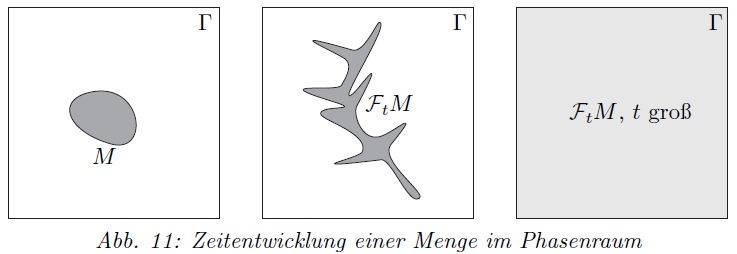
\includegraphics[width=0.8\textwidth,angle=0]{Bilder/zeitentw.png}
%\captionof{figure}{}\medskip
\label{fig:zeitentw}
\end{center}

	\anm{dabei ist das Liouville-Maß von $M$ (das Integral !) weiterhin erhalten, also $\int_M \rho_0 d\gamma = \int_{\mathcal{F}_t M} \rho_t d\gamma$ (nimmt größeres Volumen ein, aber geringere Dichte !) und man sieht, dass sich einige Teile von $M$ (Anfangszustände) annähern, andere entfernen.}\\

Das Ganze ist nicht wirklich beweisbar, man müsste immer hin und her springen zwischen den verschiedenen Aussagen, dies wäre sehr aufwendig.\\
Ein Beweisansatz von Boltzmann war die Ergodentheorie. Hier ist die Idee, dass der Gleichgewichtszustand gerade der Zustand sein sollte, den man bei einer Zeitmittelung über alle Zeiten erhält, also

\begin{equation}\label{eq:ergod}
\expval{f} = \lim_{t \rightarrow \infty} \, \frac{1}{T} \int\limits_0^T f\qty(\mathcal{F}_t \gamma) \, dt .
\end{equation}

Zu zeigen wäre nun, dass dieser Zustand für Liouville-fast-alle Anfangszustände $\gamma$ existiert und auch gleich ist (das ist ja die Definition des GGW-Zustands), das würde man als Ergodizität der Dynamik bezeichnen. Dies ist dann äquivalent dazu, dass es keine messbaren (von einem Maß, also mathematisch) Erhaltungsgrößen gibt und dass es außer den konstanten Funktionen keine weiteren messbaren Funktionen gibt.\\
Letztendlich bringt diese Theorie alleine aber keinen Erkenntnisgewinn über die Thermodynamik.

Die Erkenntnisse können uns aber trotzdem helfen. Zunächst einmal spielt sich wegen der Energieerhaltung, die ja weiterhin angenommen wird, die gesamte Bewegung im Phasenraum auf einer Energiefläche mit $E = H\qty(\gamma) = H\qty(\mathcal{F}_t \gamma) = const. \equiv U$ ab (gilt auch in Ergodentheorie). Das kommt gerade aus der Volumenerhaltung des Liouville-Maßes. Liegen aber keine weiteren offensichtlichen Symmetrien vor, die man mit dem Noether-Theorem nachweisen könnte, so folgt aus der Ergodizität, dass die zum System gehörige Dichtefunktion zeitlich konstant sein muss (diese müssen natürlich messbar sein, es soll schließlich darüber integriert werden) !

?! Zeitmittelung kann wegen Ergodentheorie ersetzt werden mit Mittelung über Gesamtheit (da jeder Zustand einmal angenommen, sollte statistische Sichtweise sein und ergibt auch Sinn) ?!

Den Erwartungswert einer Funktion/ Observablen $f$ schreibt man in diesem Fall als (nur Integration über eine Energiefläche, da $E$ als Kontrollparameter fest !)

\begin{align}\label{eq:microzust}
\expval{f}_E &:= %\int_\Gamma f(\gamma) \, d\gamma = 
\frac{\int \delta\qty(H(\gamma) - E) \, f(\gamma) \, d\gamma}{\int \delta\qty(H(\gamma) - E) \, d\gamma} := \frac{1}{\omega(E)} \int \delta\qty(H(\gamma) - E) \, f(\gamma) \, d\gamma
\\
&= \frac{1}{\omega(E)} \int_{H(\gamma)} f(\gamma) \, d\gamma = \int_\Gamma \rho_\omega(\gamma) f(\gamma) \, d\gamma \notag .
\end{align}

! nehmen alle Mikrozustände (gleich wahrscheinlich !), die angenommen werden können, und mitteln über die; Zustandssumme ist gerade das Phasenraumvolumen !

$\expval{f}_E$ heißt mikrokanonischer Erwartungswert von $f$, der Index $E$ steht einfach für die Gesamtenergie des Systems. Durch Vergleichen erhält man als Dichtefunktion die mikrokanonische Gesamtheit (singulär !)

\begin{equation}\label{eq:dichtef}
\rho_\omega(\gamma) = \frac{\delta\qty(H\qty(\gamma) - E)}{\omega(E)} = \rho_\omega = const.
\end{equation}
mit der mikrokanonischen Zustandssumme $\omega(E)$, die für die Normierung zuständig ist und aus $\expval{1}_E = 1$ bestimmt werden kann ($f = 1$, Integration über alle $\gamma \in \Gamma$).

	\anm{konstant ist hier im Sinne der Ergodentheorie gemeint, wo man sowieso nur über die Energiefläche integriert und wo deshalb die $\delta$-Funktion wegfällt.\\
	Die Motivation dieser Größe ist auch über die Forderung nach maximaler Entropie möglich, da diese gerade gegeben ist, wenn alle Zustände die gleiche Energie haben und alle Teilchenzahlen gleich wahrscheinlich sind (Rechnung siehe Hausübung 6).}

? Zustandssumme = Phasenraumvolumen ?


Man bestimmt dabei das Maß auf der Energiefläche wie bereits in \eqref{eq:energy} beschrieben über die Energieschale. Dazu wird die $\delta$-Funktion/ das Dirac-Delta benutzt, das aus der Distributionentheorie oder äquivalent aus der Hilbertraumtheorie von Johann von Neumann kommt. Die beste Darstellung dieser Funktion (so sollte man sich das vorstellen, beste Näherung; eben nicht $"$überall 0 und an einer Stelle 1$"$) ist:
\begin{equation}
\delta\qty(H(\gamma) - E) = \lim_{\epsilon \rightarrow 0} \frac{1}{\epsilon} \chi_{[E, E-\epsilon]}\qty(H(\gamma))
\end{equation}

Man kann nun zeigen, dass bei ergodischen Systemen für Liouville-fast-alle $\gamma$ die rechte Seite in \eqref{eq:ergod} existiert und da dort ebenfalls dem System eine zeitunabhängige Wahrscheinlichkeit zugeordnet wird, erhält man (Mittelwert $\rightarrow$ Erwartungswert)

\begin{equation}
\expval{f}_E = \lim_{T \rightarrow \infty} \, \frac{1}{T} \int\limits_0^T f\qty(\mathcal{F}_t \gamma) \, dt .
\end{equation}

Die mikrokanonische Gesamtheit ist also ein geeigneter Weg, den zu Bahnen $\mathcal{F}_t \gamma$ auf einer Energiefläche $H\qty(\gamma)$ gehörigen Gleichgewichtszustand zu finden (können nun also das einheitliche Grau im rechten Teil der obigen Abbildung beschreiben). Zumindest für ergodische Systeme ist also das Anknüpfen des Begriffs des Gleichgewichtszustandes an die Klassische Mechanik geglückt.

Ein Problem ist, dass es extrem schwer ist, die Ergodizität eines Systems mathematisch strikt zu zeigen. Es wird aber trotzdem oder vielleicht auch gerade deswegen angenommen, dass man beispielsweise ein Gas auch in dieser Weise beschreiben kann.


	\anm{prinzipiell muss man hier nicht das Liouville-Maß $d\gamma \equiv$ Lebesgue-Maß im Phasenraum benutzen, es wären auch möglich. Das Besondere ist aber, dass für jedes Hamilton'sche System das Maß $d\gamma$ für alle Zeiten invariant unter dem Fluss $\mathcal{F}_t \gamma$ ist (unabhängig davon, wie schlecht die Näherungen z.B. beim WW-Potential sind) ! Es hat also eine Stabilitätseigenschaft und ist daher das Mittel/ Maß der Wahl.}




	\subsection{Kanonische Gesamtheit}
Mit den Überlegungen aus dem vorherigen Abschnitt kann man nun Thermodynamik machen ! Insbesondere brauchen wir dazu aber einen Temperaturbegriff, der hier erarbeitet werden soll.

! wollen hier nicht mehr nur isoliertes/ geschlossenes System nehmen wie bei mikrokanonisch, sondern erlauben Austausch des geschlossenen mit Wärmebad (großkanonisch geht noch einen Schritt weiter, nimmt offenes System in Kontakt mit Wärmebad; daher dann Summation über Teilchenzahlen; dann $\rho = \sum\limits_{N = 0}^\infty \frac{e^{-\beta \qty(H - \mu N)}}{\Xi_\nu} = \sum\limits_{N = 0}^\infty z^N \mathcal{Z_N}$, Fugazität $z = e^{\beta \mu}$ mit großkanonischer Gesamtheit $\Xi = \Xi(T, V)$; davor war auch $\mathcal{Z} = \mathcal{Z}(T, V)$) ! Entropie als thermodynamisches Potentiel (?) nicht mehr hilfreich, da Energie nicht mehr konstant (daher dann Freie Energie genommen) !

Wir betrachten dafür wieder einen Wärmekontakt (also quasi den 0. Hauptsatz), da man die Temperatur ja aus einem Gleichgewicht zweier Systeme herleiten konnte (genauer: ein Wärmebad $B$, dessen Zustand mit $\gamma_B$ bezeichnet wird und ein beliebiges, anderes System $S$ mit $\gamma_S$). Wärmekontakt wird in der gewählten Formulierung ausdrücklich erlaubt, im Hamiltonian gibt es ja einen Wechselwirkungs-Term.

Es liegt also das System $SB$ mit zugehörigem Phasenraum $\Gamma_{Ges} = \Gamma_S \cross \Gamma_B$ in Zuständen $\gamma = \gamma_S \cross \gamma_B \in \Gamma_{Ges}$ vor, dessen Hamiltonian sich ergibt als

\begin{equation}
H(\gamma_S, \gamma_B) = H_S(\gamma_S) + H_B(\gamma_B) + V_{SB}(\gamma_S, \gamma_B) .
\end{equation}

Man kann den Wärmekontakt andererseits als Störung des aus unabhängigen Teilsystemen zusammengesetzten Systems $SB$ mit Hamiltonian $H(\gamma_S, \gamma_B) = H_S(\gamma_S) + H_B(\gamma_B)$ interpretieren (vereinfacht Beschreibung, da WW-Potentiale oft sehr kompliziert, dann liegt nämlich Produktverteilung vor). Auch das ist aber beschreibbar und überhaupt kein Problem, da das Liouville-Maß ebenfalls invariant unter Störungen ist (bereits angesprochene Stabilitätseigenschaft, leicht andere Anfangsbedingungen ändern den Endzustand nicht wesentlich).

Setzt man im Extremfall $V = 0$, so ist die Gesamtenergie $E$ (und nur die geben wir ja vor, einzige Randbedingung) nach wie vor erhalten (auch wenn Energien der einzelnen Systeme vielleicht nicht). Man kann jetzt also den Erwartungswert einer beliebigen Observablen $f$ bei fester Energie $E \equiv U$ bestimmen, was nach \eqref{eq:microzust} gerade der Berechnung der mikrokanonischen Gesamtheit entspricht, woraus folgt:

\begin{align}
\expval{f}_E &= \expval{1}_E^{-1} \int \delta\qty(H_S(\gamma_S) + H_B(\gamma_B) - E) \, f(\gamma_S) \, d\gamma_S d\gamma_B
\notag\\
&= \expval{1}_E^{-1} \int f(\gamma_S) \qty(\int \delta\qty(H_B(\gamma_B) - (H_S(\gamma_S) + E)) d\gamma_B) d\gamma_S 
\notag\\
&= \expval{1}_E^{-1} \int f(\gamma_S) \, \omega_B\qty(E-H_S(\gamma)) \, d\gamma_S
\end{align}

	\anm{$f$ muss hierfür unabhängig von Koordinaten von $B$ sein, sonst zweiter Schritt so nicht möglich, genauer heißt das $f(\gamma) = f(\gamma_S)$.}\\

Es taucht aus dem Wärmebad also nur die mikrokanonische Zustandssumme $\omega_B\qty(E-H_S(\gamma))$ auf, die hier einer Dichtefunktion entspricht (wieder durch Vergleich).\\
Da aber meist $H_S(\gamma) \neq const.$, liegt die Dichtefunktion im Allgemeinen nicht auf einer einzigen Energiefläche, was ein großer Unterschied zu vorher ist, wo $\rho_\omega = const.$ war. % (siehe \eqref{eq:dichtef}).
Insbesondere ist die Energie kein Kontroll-/ äußerer Parameter mehr (ist zwar anfangs fest, aber bleibt nicht mehr unbedingt) !

Diesen Ausdruck kann man nun in eine schönere Form bringen, indem man als Ansatz für ein Wärmebad ein Ideales Gas nimmt (ist recht einfach und bereits gut bekannt, damit kann man schön arbeiten), so hat man dort ein $N$-Teilchensystem mit $E_N = \frac{3}{2} N k_B T = N E_1$. Man kann jetzt weiter berechnen:

\begin{equation*}
\expval{f}_{E_N} = \expval{1}_{N E_1}^{-1} \int f(\gamma_S) \qty(1 - \frac{H_S(\gamma_S)}{N E_1})^{\frac{3}{2} N - 1} d\gamma_S
\end{equation*}

Im geeigneten Fall $N \rightarrow \infty$ (geeignet, da dann $S$ vernachlässigbar, das war ja Bedingung an Wärmebad) geht auch $E_N \rightarrow \infty$, aber nicht $E_1 = \frac{3}{2} k_B T = \frac{E}{N}$. Man erhält dann ($N$ in Bruch und Exponent !) den kanonischen Erwartungswert

\begin{align}
\expval{f}_\beta &:= \lim_{N \rightarrow \infty} \expval{f}_{N E_1} = \expval{1}_{N E_1}^{-1} \int f(\gamma) \, e^{-\frac{3}{2 E_1} H(\gamma)} \, d\gamma 
\notag\\
&:= \frac{1}{\mathcal{Z}} \int f(\gamma) \, e^{-\beta H(\gamma)} \, d\gamma = \int_{\Gamma_{ges}} \rho_\beta(\gamma) f(\gamma) \, d\gamma
\\
&= \int_{\Gamma_{Ges}} \rho_\beta(\gamma) f(\gamma_S) \, d\qty(\gamma_S \cross \gamma_B)\notag .
\end{align}

	\anm{es wurde einfach $\gamma_S$ durch $\gamma$ ersetzt, da $S$ ja beliebig war und der Index nur zur Unterscheidung von $B$ und $S$ war.}\\

Man erhält als neue Größen in analoger Benennung die kanonische Gesamtheit

\begin{equation}
\rho_\beta(\gamma) = \frac{e^{-\beta H(\gamma)}}{\mathcal{Z}}
\end{equation}

und die kanonischen Zustandssumme (ist ja Summe bei diskretem $\Gamma_{Ges}$, Bsp. QM)

\begin{equation}
\mathcal{Z}(\beta, V, N) = \int_{\Gamma_{Ges}} e^{-\beta H(\gamma)} \, d\gamma .
\end{equation}

Mit dem Idealen Gasgesetz ergibt sich zudem der neue Parameter als

\begin{equation}
\beta = \frac{3}{2 E_1} = \frac{1}{k_B T} .
\end{equation}

Dieser ist nach den vorherigen Rechnungen geeignet, alle Äquivalenzklassen unter Wärmekontakt zu beschreiben. Es wurde also das Ziel erreicht, einen neuen Temperaturbegriff zu finden.\\
Jedoch muss nun noch die Beziehung des kanonischen Erwartungswertes zum mikrokanonischen Erwartungswert geklärt werden, da nicht direkt klar ist, dass sie wirklich das selbe beschreiben. Das wäre jedoch gut, da der Begriff des Gleichgewichtszustandes eindeutig definiert sein sollte und der kanonische Erwartungswert ja durch Einsetzen und Rechnen aus dem mikrokanonischen hergeleitet wurde.

Ganz offensichtliche Unterschiede zeigen sich beim Vergleich der beiden Dichtefunktionen $\rho_\omega$ und $\rho_\beta$, da eine konstant ist (nur vom Kontrollparameter $E$ abhängig) und die andere nicht ($\rho_\beta$ verschwindet auch nirgendwo im Phasenraum, $\rho_\omega$ außerhalb der betrachteten Energiefläche jedoch schon).

Die Gleichheit $\expval{f}_E = \expval{f}_\beta$ muss jedoch nur im sogenannten thermodynamischen Limes mit $N, V \rightarrow \infty$ und $\frac{E}{N}$ oder $\beta$ fest gelten, was dann auch tatsächlich der Fall ist.\\
Man erhält dann als Konsequenz auch, dass in diesem Fall die kanonische Gesamtheit nur in der Nähe einer einzigen Energiefläche konzentriert ist (mikrokanonische liegt ja exakt auf einer). Das bedeutet nichts anderes, als dass die Streuung der Energie pro Teilchen $E_1$ (entspricht einer Energiedichte) für $N \rightarrow \infty$ gegen $0$ geht (ist der Fall, siehe Skript). Dabei geht jedoch nicht die Streuung von $E = N E_1$ gegen $0$ (die ist sogar $\sim N$ und geht deshalb gegen $\infty$, $N$ ist extensiv bezüglich der Varianz und intensiv bezüglich der Streuung !).

Man erhält dann gerade, dass dieser Energiewert $E = \expval{H}_\beta$ ist. Es gilt also, dass

\begin{equation}\label{key}
\expval{f}_\beta \equiv \expval{f}_{E = \expval{H}_\beta} .
\end{equation}


	\anm{die Begriffe Gesamtheit oder auch Ensemble sind eher antiquiert, man benutzt in der Quantenmechanik dann Präparationsoperator/ Dichteoperator.}\\

Übrigens entspricht die Energie $E$ des Systems natürlich genau der inneren Energie $U$, es gilt also die Beziehung (können damit die innere Energie bestimmen !)
\begin{equation}\label{key}
U = U(T, V, N) = \expval{H}_\beta .
\end{equation}
	\anm{ist logisch, da so die Dichte$\equiv$Besetzung $\rho_\beta(\gamma)$ mal die jeweilige Energie $H(\gamma)$ über alle $\gamma$ integriert wird.}

Ein allgemeines Prinzip, das zum Schluss noch vorgestellt werden soll, ist ein Trick zur Bestimmung von Erwartungswerten:

\begin{align}
\qty(\pdv{\mathcal{Z}(\beta)}{\beta})_{N,V} &= \pdv{\beta} \int e^{-\beta H(\gamma)} \, d\gamma = - \int H(\gamma) e^{-\beta H(\gamma)} \, d\gamma
\notag\\
&= - \expval{H \mathcal{Z}}_\beta = - \expval{H}_\beta \expval{\mathcal{Z}}_\beta = - \mathcal{Z} \expval{H}_\beta
\notag\\
\Leftrightarrow \expval{H}_\beta &= -\pdv{\beta}\qty(\ln \mathcal{Z}(\beta)) \label{eq:evalH}
\end{align}

	\anm{Ergebnis stimmt, weil so im Skript, aber Rechnung teilweise selber gemacht und daher unsicher; Idee ist aber, dass $H$ und $\mathcal{Z}$ unabhängig sind, also gleichzeitig bestimmbar und dann, dass $\mathcal{Z}$ konstant ist und daher $\expval{\mathcal{Z}}_\beta = \mathcal{Z}$.}\\


Ist das nicht die Boltzmann-Verteilung, eben in thermischem GGW bei fester Temperatur (also festem $\beta$) -> jup

Berechne Besetzungswahrscheinlichkeit $p_j$ (also Besetzungszahl $N_j$ geteilt durch Teilchenzahl $N$) eines gewissen Zustands/ Niveaus $j$ (charakterisiert über die zugehörige Energie $E_j$) als Erwartungswert der Funktion $\delta_{ij} = \begin{cases} 1, & i = j \\ 0, & i \neq j \end{cases}$ (ist einfach logisch, man integriert ja dabei über jeden Zustand und so wird der Beitrag aller relevanten Zustände aufsummiert -> bei endlicher Besetzung des Niveaus, was realistisch ist); das Ergebnis ist dann offenbar
\begin{equation}
p_j = \expval{\delta_{ij}}_\beta = \frac{1}{\mathcal{Z}} \sum_{\gamma: \, H(\gamma) = E_j} e^{-\beta E_j} =: \frac{g_j}{\mathcal{Z}} e^{-\frac{E_j}{k_B T}}
\end{equation}
mit dem Entartungsgrad $g_j$ des Niveaus (zählt halt einfach, wie viele Zustände diese Energie haben); dabei ist $p_j \leq 1$, weil man in $\mathcal{Z}$ ja über alle Zustände summiert (da sind insbesondere die zum Niveau $E_j$ enthalten, das sind gerade $g_j$ Stück und in den meisten Fällen noch mehr)




	\subsection{Thermodynamische Funktionen}
Es wurde ja bereits festgehalten, dass ein thermodynamisches Potential alle Informationen über ein gegebenes System enthält. Leider ist aber die bereits bekannte Funktion $U(T,V,N) = \expval{H}_\beta$ kein solches Potential, die bisherigen Erkenntnisse reichen also noch nicht zur Angabe einer solchen Funktion.

Man findet aber aus der zuvor behandelten, mikroskopischen Theorie, dass
\begin{equation}\label{key}
U = F + T S = F - T \pdv{F}{T} = F + \beta \pdv{F}{\beta} = \pdv{\beta}(\beta F) .
\end{equation}
	\anm{das $\beta$ und zweite $-$ kommen aus innerer Ableitung bei Substitution.}

Ein Koeffizientenvergleich mit \eqref{eq:evalH} ergibt dann das zu den Variablen $(T,V,N)$ gehörige thermodynamische Potential, die Freie Energie
\begin{equation}\label{key}
F(T,V,N) = F(\beta, V, N) = -\frac{1}{\beta} \ln\qty(\mathcal{Z}(\beta)) + c(V, N) .
\end{equation}


Dabei liegt noch das $c$ vor, da dieser Term bei Ableitung nach $T$ herausfällt und wir ihn somit so nicht herleiten können ! Zudem ergibt sich direkt ein großes Problem, das auch $"$Gibbs'sches Paradoxon$"$ genannt wird (da bereits Gibbs das entdeckte !): die Freie Energie ist nicht extensiv in $N$, nimmt also nicht $\sim N$ zu, was vollkommen entgegen der physikalischen Intuition ist.

Ein Vergleich mit zuvor behandelten Problemen (siehe z.B. \eqref{eq:sacktetr}) ergibt
\begin{align}\label{key}
c(V, N) &= c(N) = -N \ln(N) \approx -\ln(N!) \quad (\text{Stirling-Formel})
\\
\Rightarrow F(T, V, N) &= -\frac{1}{\beta} \ln\qty(\mathcal{Z}(\beta)) -\ln(N!)  = -\frac{1}{\beta} \ln\qty(N! \, \mathcal{Z}(\beta)) .
\end{align}
Die Klassische Mechanik liefert keine Erklärung für das Auftreten dieser Terme !


Eine bereits von Gibbs vorgeschlagene Lösung für das Problem ist es, ein normiertes Phasenraum-Maß zu verwenden und so die Terme quasi $"$reinzuschmuggeln$"$, also
\begin{equation}\label{key}
d\gamma := \frac{1}{N!} dp^3_1 \dots dp^3_N \, dq^3_1 \dots dq^3_N = \frac{1}{N!} (d\gamma)_{alt} .
\end{equation}
	\anm{bei mehreren Teilchensorten $j$ ist statt $N!$ dann $\prod_j N_j!$ zu verwenden.}


Die Begründung für diese neue Normierung des Liouville-Maßes ist, dass Konfigurationen aus $N$ Teilchen, die bis auf die Sortierung/ Nummerierung der Teilchen identisch sind, natürlich physikalisch äquivalent sind und daher zusammengefasst werden sollen. Da es davon $N!$ viele gibt, die nun in einen Zustand $\gamma$ gepackt werden, erhält man
\begin{equation}\label{key}
\gamma := \gamma_{neu} = N! \gamma_{alt} \Leftrightarrow \gamma_{alt} = \frac{\gamma}{N!}
\end{equation}
So ist sichergestellt, dass man mit den beiden Maßen das Selbe misst. Einsetzen eines Phasenraumpunktes $\gamma$ (Maß ist ja auch nur lineare Abbildung) gibt dann nämlich
\begin{equation}\label{key}
(d\gamma)(\gamma) = (d\gamma)\qty(N! \gamma_{alt}) = N! \qty(\frac{1}{N!} (d\gamma)_{alt})\qty(\gamma_{alt}) = \qty((d\gamma)_{alt})\qty(\gamma_{alt}) .
\end{equation}

Trotzdem hat man das Problem, dass dies ja nicht aus der Klassischen Mechanik an sich kommt, sondern im Nachhinein als Lösung eines Problems eingeführt wird. Das sollte eigentlich nicht der Fall sein. Man kommt also langsam an die Grenzen der mit Klassischer Statistischer Mechanik erklärbarer Phänomene.\\

Betrachtet man aber die Quantenmechanik zu diesem Thema, erhält man diese Normierung/ bzw. das richtige Phasenraum-Maß sofort im Klassischen Limes:
\begin{equation}\label{key}
d\gamma:= \frac{1}{N!} \frac{dp^3_1}{h} \dots \frac{dp^3_N}{h} \, \frac{dq^3_1}{h} \dots \frac{dq^3_N}{h} = \frac{1}{N! \, h^{3N}} (d\gamma)_{alt} .
\end{equation}
	\anm{hier wird in Einheiten mit $\hbar = 1$ gearbeitet. Dass man sich quasi nur noch Vielfache von $h$ anschaut, ist also nur Einheitenwahl ! Gleichzeitig ist es ein Hinweis auf die Quantisierung der Physik.}
%$h^{-3N}$ aus dem halbklassischen Spektralregel (aus Normierung Potentialtopf ???)

Die Begründung für den zusätzlichen Faktor $\frac{1}{N!}$ kommt in der QM dann aus der Fermi-/ Bose-Statistik und deren Vertauschungsrelationen (analoge Idee zu Gibbs).\\


In beiden Fällen erhält man dann die Formel
\begin{equation}\label{key}
F(T, V, N) = -\frac{1}{\beta} \ln\qty(\mathcal{Z}(\beta)) = -\frac{1}{\beta} \ln\qty(\int e^{-\beta H(\gamma)} \, d\gamma) ,
\end{equation}
die nun extensiv in $N$ ist und damit auch mit etwaigen Grenzfällen aus anderen Bereichen übereinstimmt.

! haben nun F bei kanonisch analog zu S bei mikrokanonisch (auch gleiche Formel mit dem ln und so !

Aus diesem thermodynamischen Potential $F$ kann man nun weitere Funktionen bestimmen, das wichtigste Beispiel ist dabei die Entropie
\begin{equation}\label{key}
S = -\pdv{F}{T} = k_B \beta^2 \pdv{\beta}\qty(-\frac{1}{\beta} \ln(\mathcal{Z})) = \dots = - k_B \int \rho_\beta(\gamma) \ln\qty(\rho_\beta(\gamma)) \, d\gamma
\end{equation}

Definiert man aber die konkave Funktion
\begin{equation}\label{key}
\eta(t) = \begin{cases} -t \ln(t), & t > 0 \\ 0, & t = 0 \\ -\infty & t < 0 \end{cases},
\end{equation}
so kann man durch folgende Definition die von $S$ geforderte Konkavität erfüllen:
\begin{equation}\label{key}
S = k_B \, \int \eta\qty(\rho_\beta(\gamma)) \, d\gamma .
\end{equation}
	\anm{Gleichheit gilt, da die 0 macht keinen Beitrag zum Integral und der Fall $\rho_\beta < 0$ nicht relevant ist, da Dichtefunktionen positiv sind (brauchen diese Teile also eigentlich gar nicht, sind nur für Konvexität da).} %, die Entropie sowieso immer relativ ist und man so argumentieren kann, dass sie vor Start der Messung o.Ä. bei $t = 0$ gar nicht sinnvoll definiert war (brauchen diese Teile also gar nicht).



	\subsection{Gibbs'sches Variationsprinzip}
In diesem Abschnitt erfolgt quasi die Rechtfertigung der eben eher aufgestellt als hergeleiteten Formel für $F$ und $S$.

Zuvor wurden $F$ als Legendre-Transformierte definiert, das kann man hier analog machen, indem man das Gibbs'sche Variationsprinzip nutzt. Man setzt dazu zunächst als Verallgemeinerung zwei Funktionale für $\hat{F}, \hat{S}$ an:
\begin{align}\label{key}
\hat{F}_H &= \inf \{U - T S\} := \inf_\rho\{\expval{H}_\beta - \frac{1}{\beta} \hat{S}(\rho)\}
\notag\\
&= \inf_\rho\{ \int \rho(\gamma) H(\gamma) \, d\gamma - \frac{1}{\beta} k_B \int \eta\qty(\rho(\gamma)) \, d\gamma \} .
\end{align}
	\anm{das $H$ im Index soll nur verdeutlichen, dass es sich um die Legendre-Transformierte von $U$ handelt.}

Man ist also auf der Suche nach der minimalen Energie und minimiert dabei über alle möglichen Dichtefunktionen $\rho$, also alle möglichen Zustände des Systems (das schließt insbesondere auch Nicht-Gleichgewichtszustände ein !).

Vergleicht man diese Ausdrücke mit denen aus dem vorherigen Abschnitt, so entsprechen diese genau den nun aufgestellten mit er Kanonischen Gesamtheit $\rho = \rho_\beta$ eingesetzt. Genau das kommt auch bei Auswertung der Infimumsbedingung heraus ! Der Vorteil ist nun aber, dass dies für beliebige Dichtefunktionen so ist und nicht nur für Gleichgewichtszustände. Das ist auch der Grund, warum im Kapitel Thermodynamik die Begriffe Freie Energie und Kanonische Gesamtheit zusammen standen.

Man sieht aus der Formel sofort, dass bei gegebenem $U = \expval{H}$ die Aufgabe der Legendre-Transformation dazu wird, die Entropie $\hat{S}$ durch Finden eines geeigneten $\rho$ zu maximieren. Die günstigsten Zustände bei einer festen Energie sind also offenbar die mit der größten Entropie !


Die Bedeutung dieses Zusammenhangs wird klar, wenn man sich folgendes vor Augen führt: möchte man sich ganze Klassische Statistische Mechanik in einer Formel merken, dann sollte es diese für Freie Energie/ Entropie geschehen, da man sich dann quasi alles andere herleiten kann (zum Beispiel wie in der Thermodynamik über Koeffizientenvergleich von Differentialen).\\

\underline{Beispiel:}\\
man betrachte nun eine Menge von Zuständen $\gamma$, die bestimmte (möglicherweise von einer Aufgabe geforderte) Eigenschaften erfüllen. Fasst man diese in der Menge $\Gamma_n \subset \Gamma$ zusammen, so erhält man die Gesamtheiten des Systems als
\begin{align}\label{key}
\rho_\omega(\gamma) &= \frac{\delta(H(\gamma) - E)}{\int_{H(\gamma) = E} d\gamma} = \frac{\delta(H(\gamma) - E)}{\int_{\Gamma_n} d\gamma} = \frac{\delta(H(\gamma) - E)}{V_{\Gamma_n}}
\\
\rho_\beta(\gamma) &= \frac{e^{-\beta H(\gamma)}}{\int_{\Gamma_n} e^{-\beta H(\gamma)} d\gamma} = \frac{e^{-\beta E}}{e^{-\beta E} \int_{\Gamma_n} d\gamma} = \frac{e^{-\beta E}}{e^{-\beta E} V_{\Gamma_n}} = \frac{1}{V_{\Gamma_n}}
\end{align}
	\anm{alle $\gamma \in \Gamma_n$ müssen die gleiche Energie $H(\gamma) = E$ haben. Das ist durchaus üblich, da diese z.B. als Kontrollparameter festgehalten werden kann oder nur begrenzt zur Verfügung steht (siehe HÜ 6.1, dort Energie im Festkörper) !}

Im zweiten Teil ist nur die Integration über $\Gamma_n$ nötig, da außerhalb ja gar keine Zustände des betrachteten Systems liegen (steckt im ersten Teil quasi in Energie-Forderung).

Setzt man diese Ausdrücke ein, so ergibt sich nun tatsächlich das gleiche Ergebnis:
\begin{align}\label{key}
\hat{S}(\rho_\omega) &= k_B \int_{\Gamma_n} \eta\qty(\rho_\omega(\gamma)) \, d\gamma = \hat{S}(\rho_\beta) = k_B \int_{\Gamma_n} \eta\qty(\rho_\beta(\gamma)) \, d\gamma
\notag\\
&= k_B \int_{\Gamma_n} -\frac{1}{V_{\Gamma_n}} \ln\qty(\frac{1}{V_{\Gamma_n}}) \, d\gamma = -\frac{k_B}{V_{\Gamma_n}} \ln\qty(\frac{1}{V_{\Gamma_n}}) \int_{\Gamma_n} d\gamma
\notag\\
&= -\frac{k_B}{V_{\Gamma_n}} \ln\qty(\frac{1}{V_{\Gamma_n}}) V_{\Gamma_n} = k_B \ln\qty(V_{\Gamma_n})
\end{align}
Die Entropie eines Systems entspricht also bis auf $k_B$ und Skalierung dem Volumen $V_{\Gamma_n}$, das dem System im Phasenraum $\Gamma$ zur Verfügung steht. Anschaulich wird das am Beispiel einer diskreten Teilmenge $\Gamma_n$: dann ist $V_{\Gamma_n}$ die Anzahl der Zustände in $\Gamma_n$.



	\subsection{Gleichverteilungssatz}
Umgangssprachlich kennt man: $" \frac{k_B T}{2}$ pro Freiheitsgrad als Beitrag zur Energie$"$.\\
In der jetzt entwickelten Sprache heißt das, dass in diesem Abschnitt eine allgemeine Aussage über den kanonischen Erwartungswert der Energie $\expval{H}_\beta$ gesucht ist.

Tatsächlich erhält man aus einer Rechnung für eine beliebige, differenzierbare Funktion $f: \Gamma \rightarrow \mathbb{R}$ (nötig zur Auswertung des Integrals: $f(p_i = \pm\infty) < \infty$) zunächst

\begin{equation}\label{key}
\expval{\pdv{f}{p_i}}_\beta = \beta \expval{f \pdv{H}{p_i}}_\beta .
\end{equation}

Für die Wahl $f = p_j$ (hatten ja, dass Impulsraum der Dualraum zum Ortsraum ist, die Impulse sind also Abbildungen), wo wird das zu

\begin{equation}\label{key}
\delta_{ij} = \beta \expval{p_j \pdv{H}{p_i}}_\beta \Leftrightarrow \expval{p_i \pdv{H}{p_i}}_\beta = \frac{1}{\beta} = k_B T .
\end{equation}

Dies sieht fast schon wie gewollt aus. Wenn man nun den allgemeinen Hamiltonian

\begin{equation}\label{key}
H(p,q) = \sum\limits_{i=1}^N \frac{p_i^2}{2 m_i(q)} + V(q) = \sum\limits_{i=1}^N \frac{1}{2} p_i \pdv{H}{p_i} + V_i(q)
\end{equation}

hinschreibt, so erhält man gerade

\begin{equation}\label{key}
\expval{H_{kin}}_\beta = \frac{N}{2} k_B T
\end{equation}

	\anm{$N$ ist hier die Anzahl der kanonischen Koordinaten (also quasi der Freiheitsgrade $n_f$), nicht unbedingt die Teilchenzahl (für $k$ Teilchen wäre $N = 3k$)}\smallskip

Das ist der sogenannte Gleichverteilungssatz.\\

Da jeder Freiheitsgrad eine kanonische Koordinate bekommt, sollte man zur Klarstellung, dass $N$ nicht immer für die Teilchenzahl steht, lieber die Anzahl der Freiheitsgrade $n_f$ verwenden (bei Helium als Atom ohne weitere Symmetrien aber z.B. einfach 3, also nur Ortsfreiheitsgrade). Testet man das Ganze z.B beim Idealen Gas, so erhält wegen der fehlenden WW und drei Impulsfreiheitsgraden gerade das altbekannte Ergebnis $\expval{H}_\beta = \frac{3}{2} N k_B T$, die Aussage wird also bestätigt.\\
Im Allgemeinen stimmt es jedoch nicht exakt, wie man empirisch ermitteln kann. Aber auch theoretisch kann man sich überlegen, dass das nicht stimmen kann: kleine Trägheitsmomente und innere Schwingungen der Atome (auch Freiheitsgrade !) wurden hier vernachlässigt, da man eine gleiche Masse überall annahm (kleine wurden vernachlässigt). Was hält einen zudem davon ab, die Atome weiter zu zerlegen in Quarks und deren Freiheitsgrade zu zählen (Spoiler: nichts. Problem.) ?

Die Lösung bringt (Überraschung) die Quantenmechanik. Hier hat man eine Quantisierung der Energie und am Beispiel der Schwingungen kann man sich überlegen, dass für $k_B T << \hbar \omega$ frieren die $n_f$ Freiheitsgrade eines Oszillators $\hbar \omega \qty(n_f +\frac{1}{2})$ ein (können nicht besetzt werden), sodass die getroffene Näherung auch die Wirklichkeit widerspiegelt.


Analog zur Herleitung oben kann man für geeignete Potentiale, die analog eine Bedingung der Form $\abs{V_i(q_i = \pm\infty)} = \infty$ erfüllen, herausfinden, dass

\begin{equation}\label{eq:virial}
\expval{q_i \pdv{H}{q_i}}_\beta = \frac{1}{\beta} = k_B T .
\end{equation}

Wegen $V_i(q) \sim q_i^\eta$, so zum Beispiel bei $V_i(q_i) = \alpha \abs{q_i}^\eta$, gilt

\begin{equation}\label{key}
q_i \pdv{H}{q_i} = \frac{1}{\eta}\pdv{V_i}{q_i} \Leftrightarrow V_i = \frac{1}{\eta}\pdv{V_i}{q_i} .
\end{equation}

Man kann nun durch Einsetzen von \eqref{eq:virial} den sogenannten Virialsatz zeigen:

\begin{equation}\label{key}
\expval{V_i}_\beta = \frac{1}{\eta}\expval{\pdv{V_i}{q_i}}_\beta = \frac{1}{\eta} k_B T .
\end{equation}



	\subsection{Beispiel}
Es erfolgt nun die Betrachtung des Standardbeispiels der Physik: dies ist harmonischen Oszillator, für den $V_i(q_i) = \alpha q_i^2$ gilt. Genauer nehme man nun $N$ gleiche Teilchen, die alle ein Harmonischer Oszillator sind und sonst keine weiteren Freiheitsgrade besitzen, man hat hier also nur die jeweils drei Orts- und Impulsfreiheitsgrade und $n_f = 3N$.\medskip\\
Zur besseren Übersicht setzen wir $p_x = p_y = p_z$, also $p_i := p, \forall i$ und analog $q_i$.

Es erfolgt nun die Berechnung einiger thermodynamischer Größen, wobei $H$ im klassischen Fall und im quantenmechanischen Fall betrachtet wird (verschiedene $\mathcal{Z}$ !):

\begin{itemize}
\item[-] klassisch:
\begin{align*}\label{key}
H_c(\gamma) &= H_c(p,q) = \sum\limits_{i=1}^{3N} \frac{p_i^2}{2m} + \frac{m\omega^2}{2}q_i^2 = \frac{3N}{2} \qty[\frac{p^2}{m} + m\omega^2q^2]% = \frac{3N}{2} \qty(\pdv{H}{p} + q \pdv{H}{q})
\\\\
\expval{H_c}_\beta &= \expval{H_{kin}}_\beta + \expval{H_{pot}}_\beta = \frac{3N}{2} k_B T + \frac{3N}{2} k_B T = 3 N k_B T
\\\\
\mathcal{Z}_c &= \int_\Gamma e^{-\beta H(\gamma)} \frac{d\gamma}{h} = \frac{1}{h} \int_\Gamma e^{-\beta \frac{3N}{2} \qty[\frac{p^2}{m} + m\omega^2 q^2]} dp dq
\\
&= \frac{1}{h} \int e^{\frac{-3N\beta}{2m} p^2} dp \int e^{\frac{-3N\beta m\omega^2}{2} q^2} dq = \frac{3 N k_B T}{h f}
\end{align*}

\begin{align*}
F_c &= -\sum\limits_{i=1}^{3N} \frac{1}{\beta} \ln\qty(\mathcal{Z}_c) = - 3N k_B T \ln\qty(\frac{3 N k_B T}{h f})
\\\\
S_c &= -\pdv{F_c}{T} = 3N k_B \ln\qty(\frac{3 N k_B T}{h f}) + 3N k_B T \frac{1}{T} = 3N k_B \qty[1 + \ln\qty(\frac{3 N k_B T}{h f})]
\\\\
C_{V, c} &= \pdv{U}{T} = \pdv{\expval{H}_\beta}{T} = 3 N k_B \; \text{ oder } \; C_{V, c} = -T \pdv[2]{F}{T} = T \pdv{S_c}{T} = T \,3N  k_B \frac{1}{T} = 3N k_B
\end{align*}

haben im System ja die Energie aller Teilchen, daher Summe bei $F$

Folgerungen für große und kleine Energien !


\item[-] quantenmechanisch (diskret; hier nur $N \equiv$ Teilchenzahl relevant):
\begin{align*}
H_q(\gamma) &= H_q(n) = \sum\limits_{i=1}^N \hbar\omega \qty[n_i+\frac{1}{2}] = N h f \qty[n+\frac{1}{2}]
\\\\
\expval{H_q}_\beta &= H_q(\gamma) ???
\\\\
\mathcal{Z}_q &= \int_\Gamma e^{-\beta H(\gamma)} d\gamma = \sum\limits_\gamma e^{-\beta H(\gamma)} = \sum\limits_{n=0}^\infty e^{-\beta N\hbar\omega \qty(n+\frac{1}{2})}
\\
&= e^{\frac{-\beta N\hbar\omega}{2}} \sum\limits_{n=0}^\infty e^{-\beta N\hbar\omega n} = e^{-\frac{N \, h f}{2 k_B T}} \frac{1}{1-e^{-\frac{N \, h f}{k_B T}}}
\end{align*}

\begin{align*}
F_q &= -\sum\limits_{i=1}^N \frac{1}{\beta} \ln\qty(\mathcal{Z}_q) = -N \frac{1}{\beta} \ln\qty(e^{-\frac{N \, h f}{2 k_B T}} \frac{1}{1-e^{-\frac{N \, h f}{k_B T}}}) = N^2 \frac{h f}{2} - N k_B T \ln\qty(\frac{1}{1-e^{-\frac{N \, h f}{k_B T}}})
\\\\
S_q &= -\pdv{F_q}{T} = \dots = N k_B \ln\qty(\frac{1}{1-e^{-\frac{N \, h f}{k_B T}}}) + N^2 \, \frac{h f}{T} \frac{1}{e^{\frac{N \, h f}{k_B T}}-1} 
\\\\
C_{V, q} &= -T \pdv[2]{F_q}{T} = T \pdv{S_q}{T} = \dots = \qty[\frac{N h f}{e^{\frac{N \, h f}{k_B T}}-1}]^2 e^{\frac{N \, h f}{k_B T}} \frac{1}{k_B T^2}
\end{align*}

kann das $N^2$ hinkommen ?

\end{itemize}

Folgerungen für große und kleine Temperaturen !


SUPER BEISPIEL IST AUFGABE 3 VON ZETTEL 6

erkennen, dass $\nu$ klein gut (dann $F$ klein und $S$ groß)



	\subsection{*Dichteentwicklung*}
Bisher wurde mathematisch eher unspannende Systeme betrachtet, die Idealen Gase ohne jegliche Wechselwirkung. Es liegt hier dann ein Hamilton

\begin{equation}\label{key}
H\qty(\gamma) = \sum\limits^N_{i=1} h\qty(\gamma_i) \Rightarrow F = -N k_B T \ln\qty(\int \exp\qty(-\beta h(\gamma_1)))
\end{equation}

Es erfolgt nun eine erste Verallgemeinerung, indem eine kleine Wechselwirkung $\Phi$ zwischen zwei Teilchen (Beispiel wäre Lenard-Jones) zugelassen wird (auch dünne Gase genannt, das heißt nämlich gerade $\frac{N}{V}$ klein). Für die kanonische Zustandssumme erhält man dann

\begin{align}\label{key}
\mathcal{Z} = \mathcal{Z}_{ideal} \cdot \mathcal{Z}_{pot}
\end{align}

Hätten eigentlich wie immer irre viele Rechnungen, aber: man hat viele gleiche Terme und kommt zudem wegen der Produkte (viele davon disjunkt) deshalb mit wenigen Integralen aus.

mache iwas mit Graphen-Kombinatorik (Produktnäherung des log ?); erhalten dann Virial-Koeffizienten (Cluster-Entwicklung)
ist zu lesen als systematische Dichteentwicklung, es kommt ja N/V vor


traditionelle Art: Entwicklung in Potenzen von $B$, da Funktion klein (haben $\beta$ klein und Potential klein für die meisten Nachbarn)
Problem dabei: wird nicht extensiv in $N$ ($\ln$ geht insbesondere gegen $\infty$ im thermodynamischen Limes, egal wie langsam er steigt !); richtig gemacht wäre wirklich Zählen, wie oft es vorkommt



	\subsection{*Simulation von Gleichgewichtszuständen*}
Hier stellt sich die Frage, ob man $e^{-\beta H}$ direkt berechnen kann. Das Problem ist wieder, dass man wahnsinnig viele Variablen hat.

Selbst im diskreten Fall $\Gamma = \qty\{\gamma\}$ mit endlich vielen, aber eben immer noch vielen Zuständen wäre es $"$hoffnungslos und unsinnig$"$, alle Werte $e^{-\beta}$ zu berechnen.

Deshalb: $"$Nachbauen der Messung$"$, man kann ja eine Stichprobe nehmen, ohne die Wahrscheinlichkeiten zu kennen und so auch Erwartungswerte berechnen. Aber nun stellt sich die Frage, wie man eine Stichprobe aus einer kanonischen Verteilung erzeugt. Daher gilt es, einen Markov-Prozess zu finden mit einem Gleichgewichtswert $e^{-\beta H}$.


Zur CÜ auch tlw.:
geht iwie darum, den kanonischen Erwartungswert zu bestimmen

werden von rundungsfehlern erschlagen, wenn wir lineare algebra versuchen (da die WS bei zu vielen Teilchen durch Nachkommastellen beschränkt, ist nicht mehr angebbar und die Gesamt-WS wird quasi Zufallszahl !)

Zustandsraum so groß, dass Listung von WS nicht mehr sinnvoll; analog ist es eben bei Berechnung des Ensembles eines Systems (Beispiel Magnetfeld)


Problem numerische Integration: Anzahl der Stützstellen nimmt enorm zu; daher Monte-Carlo (Fehler der Ordnung $\frac{1}{\sqrt{N}}$, kann also bis auf bestimmten Fehler genau bestimmen), wo man Werte im Intervall bestimmt und den Mittelwert nimmt


haben extrem unterbestimmtes Problem, da nur $N$ Bedingungen aus Zusammenhang $P$ und $\rho$, aber $N^2$ Matrixelemente (finden immer irgendeine Lösung); aber wie schränke ich jetzt noch besser ein (sind ja bei weitem nicht alle Lösungen sinnvoll !) ? Antwort ist detailliertes Gleichgewicht; kriege dadurch transponiertes Matrixelement direkt mit, bei Anwendung der Matrix $P$ auf $\rho$ (also $(P\rho)(y)$)
Wenn wir Erreichbarkeit für $P$ sichern (jeder Punkt kann in endlich vielen Schritten von jedem anderen Punkt erreicht werden), dann ist der Eigenwert 1 nicht entartet (Perron-Frobenius); kann Fehler der Simulation über n-te Potenz des größten Eigenwertes von $P$ (Vergleich: WS, in einem Würfelspiel nie die 6 zu kriegen); dieser größte EW wird oft empirisch bestimmt, Fehler hängt ab von Differenz zu 1
Problem: müssen trotzdem exponentiell viele $P(\cdot|\cdot)$ bestimmen, haben nichts gewonnen; außer wir können lokale WW annehmen (möglich, wenn die Zustandsmenge genügend Struktur hat; müssen also nächste Nachbarn klassifizieren)
Können dann also lokal eine Simulation bauen und so $P$ berechnen. Beispiel Spin: Übergangs-WS zu anderem Spin hängt von Energiegewinn dabei ab (ist gerade lokal), machen also stochastisches Update der einzelnen Spins ($"$stochastischer Zellularautomat$"$)

zu Übungsaufgabe: nehmen statt Spin $=\pm 1$ bei Magneten dann beliebige Größe, die z.B. 0,1 annehmen kann (unbesetzt und besetzt) also ein sogenanntes Gittergas; arbeiten da bei fester Teilchenzahl, diese Erhaltung muss dann natürlich lokal gesichert werden (arbeiten ja nur lokal; ein Weg wäre Vertauschung von Nachbarn)
in seiner Skizze sieht man, dass wenn die im Rechteck getauscht werden, Energie gewonnen wird (bevorzugt bei niedriger Temperatur); alle Paarvertauschungen durchführen, für die Energie lokal kleiner wird (schauen nur lokal an, global interessiert und hier nicht, auch Energie nur lokal relevant); meinen nicht mehr physikalischen Spin dann !

Was ist nun mit der Lücke des EW zu 1, wie schnell ist die Konvergenz da (insbesondere als Funktion von $L$) ? Wäre doof, wenn erreicht, wegen Entartung bei Gleichheit !

Auch in FKP relevant: hat man Grundzustand und dann ne Gap oder etwas kontinuierliches ?

zum Glück Theorem: Lücke bleibt offen, können Abschätzung gleichmäßig in $L$ (Gitterlänge, also Maß für Systemgröße) machen

bei Phasenübergang geht Gap gegen 0, dann große Fluktuationen


	\subsection{*Phasenübergang im Ising-Modell*}
Wie in der Überschrift angedeutet, wird hier nur ein Modell für Phasenübergänge behandelt, nämlich das Ising-Modell (wurde bereits angesprochen bei Spin-Flips im vorherigen Abschnitt).

bekannt war das Weiss-Modell (mean field, in der QM Heisenber-Modell; Weiss'sche Bezirke ??); Quatsch, weil so WW von zwei Teilchen beeinflußt von Teilchenanzahl, aber ist eben gut zu berechnen
daraufhin Lenz zu Ising: versuch mal realistischer eine lokale WW; Ising hat es aber vergeigt

Technik von Ising funktioniert eigentlich, hier Vorstellung des 1D-Falls mit nächste-Nachbarn-WW
dann mit $h$ für den lokalen Hamiltonian

\begin{align}\label{key}
\rho(s_1, \dots, s_L) = \frac{1}{\mathcal{Z}} \exp\qty(-\beta \qty[\sum\limits_i h(s_i, s_{i+1}) + h_{Rand}(s_1, s_L)])
\\
= \frac{1}{\mathcal{Z}} e^{-\beta h_{Rand}} \prod_{i=1}^{L-1} T(s_i, s_{i+1}) = \frac{1}{\mathcal{Z}} e^{-\beta h_{Rand}} \prod_{i=1}^{L-1} e^{-\beta h(s_i, s_{i+1})}
\end{align}

mit der Transfermatrix $T$ (wurde translationsinvariant gewählt, also für alle Gitterplätze gleich !)

$P$ als Projektor (nicht orthogonal aber !), der wird einfach als dyadisches Produkt aus Eigenvektoren aufgebaut; erster Eigenwert ist der Perron-Frobenius-EW, der andere Teil geht also exponentiell gegen 0 (Rand ist hier egal, spielt keine Rolle, da die eben vernachlässigt werden können)

der EW hat ganz tolle Eigenschaften (bei Störung der Matrix auch analytische Funktion, also keine Knicks in irgendwelchen Ableitungen und man kann Potenzreihenentwicklung machen); ganz easy mit analytischem Funktionalkalkül, drücke den Projektor durch ein Cauchy-Integral aus

$T > 0$ vorausgesetzt (dann hat Matrix Nulleinträge nämlich; gerade nur mit Plussen oder nur Minussen), da sonst Nulleinträge in Matrix und dann hat man eben nur wenige Möglichkeiten


man sah es stark als Problem an, dass das nicht klappte in 1D; man kann aber Limiten vertauschen (Ableitung und thermodynamischen)

thermodynamischer Limes führt zu Phasenübergang !



$B$ als Magnetfeld oder im Gittergas-Modell dann chemisches Potential

Peierls-Argument: nehme Trennlinien von Regionen mit unterschiedlichen Spins (Klumpen), die werden Konturen genannt; die kosten immer Energie und die ist proportional zur Länge der Kontur (lange sind also unwahrscheinlich)

bei hohen (eher normalen) Temperaturen hat man im Prinzip Gauß-Verteilung der Magnetisierung um den Nullpunkt (das kommt gerade von den Klumpen); bei tiefen Temperaturen kann man gerade kanonische WS-Verteilung erhalten, die nicht mehr um 0, sondern bei $\pm 1$ konzentriert ist ! das ist dann gerade Spin-Flip, dort haben alle gleiche Energie auch

in der Theorie brauchen wir einen Symmetriebruch für einen Phasenübergang; lege dazu z.B. kleines B-Feld an ($"$symmetrie-brechendes Feld$"$)

muss Außenspin wählen ! das wird der Symmetriebruch dann, weil die Konturen auf dem Rand enden müssen, dort liegt ja nur eine Spinart vor (können nur geschlossene nehmen dann); Konturen sind also entweder geschlossen oder gehen von Rand zu Rand

können Konturen auch eine Richtung geben (dass minus immer links liegt z.B.); können die lokal ja immer einzeichnen, interessant sind insbesondere Knicke (müssen es aber eindeutig machen, was ist wenn sich zwei treffen oder so ?)

haben quasi Abbildung zwischen Modellen (von Spins zu Konturen), müssen dabei aber natürlich vorsichtig sein und das gut überprüfen

können nun innen oder außen relativ zu einer Kontur definieren; haben primitive Abschätzung der Fläche durch die Konturenlänge (grob, passt aber hier)

wenn ich Peaks unterscheiden will, muss man irgendwas unterscheiden, wir nehmen hier den Außenspin

lange Konturen sind unwahrscheinlich natürlich



	\subsection{*Entropie*}
Maß dafür, wie weit System vom GGW-Zustand weg ist; bzw. wie viele GGW-Zustände zur Verfügung stehen ?

Ist Art Zeitbegriff (deswegen begann erst mit dem Urknall die Zeit, vorher keine Objekte, die $"$ungeordnet$"$ wären)

Informations-Entropie ist Verteilungsgröße

Aus Übung: Berechnung $S =k_B \hat{S}(\rho_\beta) = k_B \ln\qty(V_\Gamma)$ auf jeden Fall was anderes als Volumen (war nur Spezialfall vermutlich) -> ne, passt ! (Gibbs-Entropie): nehmen dabei das Phasenraumvolumen $V_\Gamma$, da das ein Maß für Anzahl der Lösungen ist, die ja in $\Gamma$ drin sind !!! Ein Punkt hat ja z.B. nur einen möglichen Zustand und deshalb keine Entropie. Entropie ist Maß dafür, ob Systeme im thermischen Gleichgewicht sind (Formel aus Übung umstellen, Systeme sollen ja gleiche Temperatur haben). Können auch Differential der Energie betrachten, dann erhält man die Formel für $T$ aus $dE = \pdv{E}{S} dS + \dots$, sodass $\frac{1}{T} = \pdv{E}{S}$ folgt.

Mit einer WS-Verteilung $P$, die Elementen einer anderen Menge $M$ jeweils WS zuordnet, gilt dann $S(P) = - \sum\limits_{x \in M} P_x \log_2(P_x)$

Entropie ist erstmal Zustandsgröße; reversibel im Sinne von Isoflächen der Entropie bei adiabatischen Prozessen; System braucht sonst Hilfe von außen, um wieder zurück zu kommen; reversibel ist keine Zustandsgröße, müssen da unterscheiden (Zusammenhang aber ok, verständlich)

Boltzmann verwendet das auch als Zustandsgröße, darin taucht das Phasenraumvolumen eines Makrozustandes auf; besagt im Prinzip, dass Entwicklung eines Systems der Wahrscheinlichkeit folgt (die im Phasenraumvolumen gemessen wird); ist ne gute und klare Idee, aber knifflig zu präzisieren (haben im Prinzip ja Unsicherheit/ Unschärfe bei Wahl der makroskopischen Variablen)

Problem: brauche glatte Energiedichte, haben ja eigentlich in der Form, dass immer 0, außer bei Teilchen (dort sehr groß dann); das ist aber doof so, da man dann mikroskopisch (also auf ganz kleinen Gebieten, wo kein Teilchen drin) Probleme kriegt, wo dann nur Gebiete vom Maß 0 auftreten (aber was ist dann ein sinnvoller Volumenbegriff ?); man macht dann oft gerne so etwas wie Zellteilung (aber dann auch Unsicherheit bei Zuordnung von mikroskopischen zu makroskopischen Zuständen); Energiedichte will Ort und Energie (QM macht da aber Probleme !)

Boltzmann: betrachte Dichte im Ein-Teilchen-Phasenraum

Entropie als Maß für Phasenraumvolumen (soll dann eben jeweils zunehmen)

geordnete Familien von Zuständen brauchen wenig Phasenraumvolumen (also wenige mögliche Gleichgewichtszustände); aber viele verschiedene Möglichkeiten, einen ungewöhnlichen (eben ungeordneten) Zustand zu realisieren

hängt aber auch davon ab, wie ich die Zustände klassifiziere (machen das makroskopisch, daher diese Sichtweise; müssen unsere Version von Ordnung definieren); mikroskopisch sind alle Zustände gleichverteilt !!!

aus dieser H-Gleichung kommt die Boltzmann-Gleichung


Zusammenhang zu Unordnung hängt von Sichtweise ab, also von den Größen, die wir messen (mitteln ja z.B. meist nur, da Phasenraum so groß)

Gibbs betrachtet die mikroskopische Entropie einer Phasenraumverteilung; nehmen an, dass mikrokanonisch die Dichte in einer Energieschale konstant ist, dann folgt mit $-k_B \log(\rho) = k_b \log(V_\Gamma) \sim$ Entropie; nimm allgemeiner den Mittelwert davon, also $S(\rho) = \int \eta\qty(\rho(\gamma)) \, d\gamma$ mit einer konvexen (?) Funktion $\eta$, die vorher schon einmal erwähnt wurde (nicht mehr taylor-approximierbar, da unendliche Steigung im Nullpunkt); dann ist also $S$ ein Verteilungsparameter, der wegen der Dichte quasi die $"$Gemischtheit$"$ des Systems/ der Dichte misst (geht nicht linear auch !); ist aber keine messbare Größe, wie wir es vorher hatten ! die typischen thermodynamischen Größen sind Erwartungswerte, Zufallsvariablen etc. (ist hier gar nicht so, können das nicht einem Punkt oder so zuordnen (?)); wesentliche Leistung ist Gibbs'sches Variationsprinzip, wo auch die freie Energie rauskommt (really ? oder meint er, wie)

Dualraum zu Dichtematrizen ist Raum der Observablen/ Operatoren und dazwischen kann man mit Legendre wechseln (ob da min oder max steht ist nur VZ-Konvention); $T \, dS$ oder $\frac{1}{\beta} S(\rho)$ geht beides, beim zweiten ist $S$ eben nur dimensionslos


von Neumann (eigentlich Vater der QM, weil er gesamten Formalismus gebaut hat, aber weniger beachtet) hat das Analogon in der QM gefunden: $S(\rho) = \tr \eta(\rho)$, wobei man $\eta$ dann im Funktionalkalkül auswerten muss; in der Spektralzerlegung von $\rho$ erhält man es dann als Funktion der Koeffizienten vor den Projektoren


Claude Shannon stellte die Entropie in der Informationstheorie auf in seinem quasi Manifest für die Digitalisierung: effizientere Nutzung von Bits durch Umschreiben des Textes (manche Buchstaben/ Wörter kommen viel häufiger vor als andere, nehmen aber gleichen Speicherplatz ein ! Versehe also häufig vorkommende Sachen mit kleinem Speicherplatz, unabhängig von der Quelle, die als unabhängig gleichverteilt angenommen wird; daher scheißt Google Translate auf Grammatik und ordnet nur nach Häufigkeit die jeweiligen Sätze zu); hier taucht dann Formel analog zu Gibbs auf (nur mit Zweier-log, da ja bei Bits), bei optimaler Codierung braucht man $S(p) = \sum\limits_{x \in X} \eta\qty(p(x))) = \sum\limits_{x \in X} -p(x) \log_2\qty(p(x))$ Bits pro Zeichen zur Codierung der Quelle (sei $X$ ein zugehöriges Alphabet und $p(x)$ die Wahrscheinlichkeit für das Symbol $x \in X$); minimale Entropie bei bester Codierung bei vorgegebener Irrtumswahrscheinlichkeit; kann aber natürlich nicht alle fehlerfrei codieren dann, nehmen seltene Irrtümer in Kauf
zur Fehlervermeidung: schicke Signal dreimal und mache Mehrheitsentscheid über die drei Bit-Werte; wenn alle vorkommenden Dinger gleich wahrscheinlich sind, dann nummeriert man einfach durch mit z.B. binärer Zahlenfolge; muss dann natürlich Codebuch verteilen zum Austausch, das ist an Shannon-Grenze sehr aufwendig (daher oft weniger effiziente genommen, aber eben mit kleinerem Codebuch); Bildtelefonie beruht darauf, dass man Gesichter toll codieren kann (haben ja ein erwartetes Muster darin, sehen immer irgendein Gesicht)



\section*{Ergänzungen, die erstmal nicht zuzuordnen waren}

gleiche Energie um 1kg Wasser um 1°C zu erhöhen, kann dieses kg ca. 400m in die Luft heben (Wärmeäquivalent -> ganz schwer, Kalorien zu verbrennen, auch mit Sport, davon ist eher wichtig, den Stoffwechsel anzuregen)

Sinn 3.3: kann trotzdem überall hin (finde Nullkurve zu jedem Punkt), aber es wird eben keine Fläche von Nullkurven aufgespannt (da kein Gradient) -> soll eben veranschaulicht werden

bezahle Freie Energie beim Energieversorger, nicht innere

Go-Board aus PBS SpaceTime als Beispiel bei Entropie (Mikrozustände)
-> als Veranschaulichung: wie gut ist Energie verteilt (S klein, wenn auf engem Raum und groß, wenn gut verteilt)

doppelte Anwendung Fourier heißt Spiegelung im Phasenraum (müssen viermal machen, damit es exakt das gleiche gibt, sonst eben Funktion mit negativem Argument)

Untersuchen von Wirtschaft mit Legendre-Trafos ($"$Temperatur$"$ von Märkten)

Gleichverteilung muss präpariert werden, nicht gottgegeben (sondern symmetriegegeben) !

Spin-Statistik-Theorem $\rightarrow$ kommt von Pauli, besagt dass Fermionen (also Teilchen, die der Fermi-Statistik genügen) Spin-$1/2$-Teilchen sind und Bosonen Spin-1-Teilchen


kanonische Gesamtheit aus Statistik von Teilsystemen (aus Mikrozuständen quasi)

reiner Zustand (soll $\gamma_0$ heißen) ist hier $\rho(\gamma) = \delta(\gamma - \gamma_0)$, dann ist $\expval{f}_\rho = f(\gamma_0)$



sehr nices Veritasium Video: jeder Zustand eines Systems ist gleich wahrscheinlich (mit gleicher Energie, gleicher Teilchenzahl etc.; könnten vermutlich eher Konfiguration sagen); Entropie = Unordnung kommt dann daher, dass geordnete Zustände einfach viel unwahrscheinlicher sind als ungeordnete, weil es einfach viel weniger davon gibt!



\end{document}